% ============================================================
%  BÁO CÁO ĐỒ ÁN MÔN HỌC: DEEP LEARNING
%  Đề tài: Phát hiện té ngã bằng Fine-tune YOLO11
% ============================================================
\documentclass[12pt, a4paper]{article}

% ── Encoding & Language ─────────────────────────────────────
\usepackage[utf8]{inputenc}
\usepackage[T5]{fontenc}
\usepackage[vietnamese,english]{babel}

% ── Page Layout ─────────────────────────────────────────────
\usepackage[
  top=2.5cm, bottom=2.5cm,
  left=3cm,  right=2.5cm
]{geometry}
\usepackage{setspace}
\usepackage{indentfirst}
\onehalfspacing

% ── Math ────────────────────────────────────────────────────
\usepackage{amsmath, amssymb, amsthm}

% ── Graphics & Figures ──────────────────────────────────────
\usepackage{graphicx}
\usepackage{float}
\usepackage{subcaption}
\graphicspath{{./}{docs/}}         % hỗ trợ build từ thư mục docs hoặc từ root project

% ── Tables ──────────────────────────────────────────────────
\usepackage{booktabs}
\usepackage{multirow}
\usepackage{array}
\usepackage{tabularx}

% ── Code Listing ────────────────────────────────────────────
\usepackage{listings}
\usepackage{xcolor}

\definecolor{codegreen}{rgb}{0,0.6,0}
\definecolor{codegray}{rgb}{0.5,0.5,0.5}
\definecolor{codepurple}{rgb}{0.58,0,0.82}
\definecolor{backcolour}{rgb}{0.97,0.97,0.97}

\lstdefinestyle{mystyle}{
  backgroundcolor=\color{backcolour},
  commentstyle=\color{codegreen},
  keywordstyle=\color{blue}\bfseries,
  numberstyle=\tiny\color{codegray},
  stringstyle=\color{codepurple},
  basicstyle=\ttfamily\footnotesize,
  breakatwhitespace=false,
  breaklines=true,
  captionpos=b,
  keepspaces=true,
  numbers=left,
  numbersep=5pt,
  showspaces=false,
  showstringspaces=false,
  showtabs=false,
  tabsize=2,
  frame=single,
  rulecolor=\color{black!20}
}
\lstset{style=mystyle}

% ── Hyperlinks ──────────────────────────────────────────────
\usepackage[
  colorlinks=true,
  linkcolor=blue!70!black,
  citecolor=green!50!black,
  urlcolor=blue
]{hyperref}

% ── Caption ─────────────────────────────────────────────────
\usepackage{caption}
\captionsetup{font=small, labelfont=bf}

% ── Header / Footer ─────────────────────────────────────────
\usepackage{fancyhdr}
\setlength{\headheight}{14pt}
\pagestyle{fancy}
\fancyhf{}
\fancyhead[L]{\small Đồ án môn Deep Learning}
\fancyhead[R]{\small Phát hiện té ngã - Fine-tune YOLO11}
\fancyfoot[C]{\thepage}
\renewcommand{\headrulewidth}{0.4pt}

% ── Miscellaneous ───────────────────────────────────────────
\usepackage{enumitem}
\usepackage{multicol}
\usepackage{tikz}
\usetikzlibrary{shapes.geometric, arrows.meta, positioning, fit}

% ============================================================
\begin{document}
\hypersetup{pageanchor=false}

% ──────────────────────────────────────────────────────────
%  TRANG BÌA
% ──────────────────────────────────────────────────────────
\begin{titlepage}
  \centering
  \vspace*{1cm}

  {\Large \textbf{TRƯỜNG ĐẠI HỌC CÔNG THƯƠNG THÀNH PHỐ HỒ CHÍ MINH}}\\[0.3cm]
  {\large \textbf{KHOA CÔNG NGHỆ THÔNG TIN}}\\[0.5cm]
  \rule{\textwidth}{1.5pt}\\[0.5cm]

  \vspace{1.5cm}
  {\LARGE \textbf{BÁO CÁO ĐỒ ÁN MÔN HỌC}}\\[0.3cm]
  {\Large \textbf{DEEP LEARNING}}\\[2cm]

  {\huge \bfseries
PHÁT HIỆN TÉ NGÃ BẰNG\\[0.25cm]
PHƯƠNG PHÁP FINE-TUNE\\[0.25cm]
YOLO11\\[0.25cm]
}

  \vspace{2cm}
  \begin{flushright}
  \textbf{Giảng viên hướng dẫn: Huỳnh Thái Học}\\[0.8cm]
  \textbf{Nhóm : 6}\\[0.6cm]
  Trình Quốc An - 2001230006\\[0.4cm]
  Nguyễn Huy Hoàng - 2001230264\\[0.4cm]
  \end{flushright}

  \vfill
  {\large Thành phố Hồ Chí Minh, tháng 06 năm 2026}
\end{titlepage}

\hypersetup{pageanchor=true}
\pagenumbering{roman}

% ──────────────────────────────────────────────────────────
%  MỤC LỤC
% ──────────────────────────────────────────────────────────
\tableofcontents
\newpage

\listoffigures
\listoftables
\newpage
\pagenumbering{arabic}

% ============================================================
%  CHƯƠNG 1 — GIỚI THIỆU
% ============================================================
\section{Giới thiệu}

\subsection{Đặt vấn đề}
Té ngã là một trong những tai nạn thường gặp ở người cao tuổi, bệnh nhân sau phẫu thuật và người có hạn chế về vận động.
Khi không được phát hiện kịp thời, té ngã có thể gây ra các hậu quả nghiêm trọng như gãy xương, chấn thương đầu hoặc mất khả năng vận động.
Trong một số trường hợp, người bị té ngã không thể tự gọi trợ giúp, nhất là khi ở một mình hoặc ở khu vực ít người quan sát.

Hiện nay, việc giám sát té ngã vẫn thường dựa vào người chăm sóc, camera an ninh hoặc các thiết bị đeo trên cơ thể.
Các phương pháp này có những hạn chế nhất định.
Quan sát thủ công khó duy trì liên tục trong thời gian dài, còn thiết bị đeo phụ thuộc vào việc người dùng có mang thiết bị đúng cách hay không.
Nếu thiết bị hết pin, bị tháo ra hoặc không được sử dụng thường xuyên, hệ thống có thể bỏ sót sự cố.

Vì vậy, phát hiện té ngã bằng thị giác máy tính là một hướng tiếp cận đáng quan tâm.
Thông qua hình ảnh từ camera, hệ thống có thể phân tích tư thế người và nhận biết các trạng thái bất thường của cơ thể.
Với sự phát triển của các mô hình Deep Learning, đặc biệt là các mô hình phát hiện đối tượng và ước lượng tư thế người, bài toán phát hiện té ngã có thêm nhiều khả năng cải thiện về độ chính xác và tính tự động.

\subsection{Mục tiêu đề tài}
Đề tài hướng đến việc xây dựng và đánh giá một quy trình fine-tune mô hình YOLO11-Pose cho bài toán phát hiện té ngã dựa trên tư thế người.
Các mục tiêu cụ thể gồm:
\begin{itemize}[nosep]
  \item Tìm hiểu cơ sở lý thuyết về Object Detection, YOLO11-Pose và Human Pose Estimation.
  \item Chuẩn bị dữ liệu theo định dạng YOLO Keypoint phù hợp với mô hình YOLO11-Pose.
  \item Fine-tune mô hình pretrained \texttt{yolo11s-pose.pt} trên dữ liệu té ngã.
  \item Đánh giá kết quả huấn luyện thông qua các chỉ số định lượng và phân tích một số trường hợp dự đoán thực tế.
\end{itemize}

\subsection{Phạm vi đề tài}
Trong phạm vi đồ án môn học, đề tài được giới hạn như sau:
\begin{itemize}[nosep]
  \item \textbf{Mô hình:} Sử dụng pretrained \texttt{yolo11s-pose.pt} (Ultralytics).
  \item \textbf{Dữ liệu:} Sử dụng tập dữ liệu ảnh có annotation dạng bounding box và keypoint của người.
  \item \textbf{Phương pháp:} Fine-tune từ mô hình đã pretrained, không huấn luyện mô hình từ đầu.
  \item \textbf{Đánh giá:} Tập trung vào kết quả trên tập validation/test và một số mẫu inference minh họa.
  \item \textbf{Giới hạn:} Chưa triển khai thành ứng dụng hoàn chỉnh và chưa xử lý video theo thời gian thực.
\end{itemize}

\subsection{Cấu trúc bài báo cáo}
Báo cáo gồm sáu chương.
Chương~1 giới thiệu bối cảnh, mục tiêu, phạm vi và cấu trúc của đề tài.
Chương~\ref{sec:theory} trình bày cơ sở lý thuyết về Object Detection, YOLO11-Pose, Human Pose Estimation, fine-tuning và các độ đo đánh giá.
Chương~\ref{sec:dataset} mô tả dataset, định dạng annotation, thống kê dữ liệu và các bước tiền xử lý.
Chương~\ref{sec:pipeline} trình bày pipeline fine-tune, cấu hình thực nghiệm và quá trình huấn luyện.
Chương~\ref{sec:experiments} trình bày kết quả thực nghiệm, đánh giá mô hình và phân tích lỗi.
Chương~\ref{sec:conclusion} tổng kết kết quả đạt được, nêu hạn chế và đề xuất hướng phát triển.

% ============================================================
%  CHƯƠNG 2 — CƠ SỞ LÝ THUYẾT
% ============================================================
\section{Cơ sở lý thuyết}
\label{sec:theory}

\subsection{Object detection và one-stage detector}

\subsubsection{Tổng quan object detection}
Object Detection là bài toán xác định trong ảnh có những đối tượng nào và vị trí của từng đối tượng nằm ở đâu.
Khác với bài toán phân loại ảnh, trong đó mô hình chỉ dự đoán nhãn chung cho toàn bộ ảnh, Object Detection cần trả về đồng thời nhãn lớp (class label) và vùng chứa đối tượng.
Vùng chứa này thường được biểu diễn bằng bounding box gồm tọa độ tâm, chiều rộng và chiều cao của hộp bao quanh đối tượng.

Đầu ra của một mô hình Object Detection thường gồm ba thành phần chính: bounding box, nhãn lớp và độ tin cậy (confidence score).
Bounding box cho biết vị trí đối tượng trong ảnh, nhãn lớp cho biết đối tượng thuộc loại nào, còn confidence score thể hiện mức độ chắc chắn của mô hình đối với dự đoán đó.
Trong các hệ thống thị giác máy tính, Object Detection là bước nền tảng cho nhiều bài toán phức tạp hơn như theo dõi đối tượng, nhận dạng hành động, phân tích hành vi và ước lượng tư thế người.

Đối với bài toán phát hiện té ngã, Object Detection giúp xác định vị trí người trong khung hình trước khi phân tích sâu hơn về tư thế.
Khi kết hợp với Pose Estimation, mô hình không chỉ biết người xuất hiện ở đâu mà còn có thể dự đoán các điểm keypoint trên cơ thể, từ đó hỗ trợ nhận biết các tư thế bất thường như nằm, ngã hoặc mất thăng bằng.

\subsubsection{Two-stage detector và one-stage detector}
Các phương pháp Object Detection hiện đại thường được chia thành hai nhóm: Two-stage Detector và One-stage Detector.
\begin{itemize}
  \item \textbf{Two-stage Detector} như Faster R-CNN~\cite{ren2015faster}: mô hình tạo ra các vùng đề xuất có khả năng chứa đối tượng, sau đó phân loại và tinh chỉnh bounding box cho từng vùng. Cách tiếp cận này thường cho độ chính xác tốt nhưng tốc độ suy luận chậm hơn do phải xử lý qua hai giai đoạn.
  \item \textbf{One-stage Detector} như YOLO~\cite{redmon2016yolo} và SSD: mô hình dự đoán trực tiếp bounding box, nhãn lớp và confidence score trong một lần forward pass. Cách tiếp cận này có tốc độ nhanh hơn, phù hợp với các bài toán cần xử lý gần thời gian thực.
\end{itemize}

Trong đề tài này, YOLO11-Pose thuộc nhóm One-stage Detector.
Ưu điểm về tốc độ của YOLO phù hợp với bài toán phát hiện té ngã, vì hệ thống giám sát cần phản hồi nhanh khi có sự cố xảy ra.

\subsubsection{Anchor-based và anchor-free detector}
Trong các mô hình Object Detection, một điểm khác biệt quan trọng là cách mô hình dự đoán bounding box.
Các mô hình anchor-based sử dụng một tập các anchor box được định nghĩa trước với nhiều kích thước và tỷ lệ khác nhau.
Mô hình học cách điều chỉnh các anchor box này sao cho khớp với đối tượng thật trong ảnh.
Cách làm này hiệu quả trong nhiều trường hợp nhưng phụ thuộc vào việc thiết kế anchor box phù hợp với dữ liệu.

Ngược lại, các mô hình anchor-free không cần sử dụng anchor box cố định.
Mô hình dự đoán trực tiếp vị trí và kích thước của bounding box dựa trên đặc trưng ảnh.
YOLO11 sử dụng hướng tiếp cận anchor-free, giúp đơn giản hóa quá trình huấn luyện và giảm sự phụ thuộc vào các tham số thiết kế thủ công.
Điều này có lợi khi áp dụng mô hình cho các bộ dữ liệu có tư thế người đa dạng, chẳng hạn dữ liệu té ngã với nhiều góc nhìn và dáng người khác nhau.

% ─────────────────────────────────────────
\subsection{Tổng quan họ mô hình YOLO}

YOLO (You Only Look Once) là họ mô hình phát hiện đối tượng một giai đoạn, được thiết kế để dự đoán bounding box và nhãn lớp trực tiếp trong một lần lan truyền qua mạng.
Từ phiên bản đầu tiên năm 2016, YOLO đã trải qua nhiều cải tiến về backbone, cơ chế dự đoán, tốc độ suy luận và khả năng triển khai trên thiết bị thực tế.

\begin{table}[H]
  \centering
  \caption{Tóm tắt một số phiên bản tiêu biểu của họ mô hình YOLO}
  \label{tab:yolo_history}
  \begin{tabularx}{\textwidth}{@{}l>{\raggedright\arraybackslash}X>{\raggedright\arraybackslash}X@{}}
    \toprule
    \textbf{Phiên bản} & \textbf{Đặc điểm nổi bật} & \textbf{Ý nghĩa cải tiến} \\
    \midrule
    YOLOv1 (2016) & Đề xuất cách tiếp cận one-stage detector & Dự đoán trực tiếp bounding box và class trong một lần xử lý ảnh \\
    YOLOv3 (2018) & Multi-scale detection, Darknet-53 & Cải thiện khả năng phát hiện đối tượng ở nhiều kích thước \\
    YOLOv5 (2020) & Triển khai bằng PyTorch, dễ huấn luyện và triển khai & Góp phần phổ biến YOLO trong các ứng dụng thực tế \\
    YOLOv8 (2023) & Anchor-free, decoupled head & Đơn giản hóa thiết kế và cải thiện hiệu quả huấn luyện \\
    YOLO11 (2024) & C3k2, C2PSA, hỗ trợ nhiều tác vụ thị giác máy tính & Cải thiện cân bằng giữa tốc độ và độ chính xác \\
    YOLO12 (2025) & Kiến trúc chú trọng attention & Khai thác attention trong bài toán phát hiện đối tượng thời gian thực \\
    YOLO26 (2026) & Tối ưu cho edge AI và suy luận nhanh hơn & Hướng đến triển khai thực tế trên thiết bị tài nguyên hạn chế \\
    \bottomrule
  \end{tabularx}
\end{table}

Trong phạm vi đề tài này, mô hình được sử dụng là \texttt{yolo11s-pose.pt}.
Mặc dù đã có các phiên bản mới hơn, YOLO11-Pose vẫn phù hợp với bài toán phát hiện té ngã vì có sẵn biến thể Pose Estimation, hỗ trợ huấn luyện keypoint tùy chỉnh và được tích hợp trực tiếp trong hệ sinh thái Ultralytics.

% ─────────────────────────────────────────
\subsection{Kiến trúc YOLO11-Pose}
\label{subsec:yolo11_arch}

YOLO11-Pose là biến thể của YOLO11 được thiết kế cho bài toán Human Pose Estimation.
Thay vì chỉ dự đoán bounding box và nhãn lớp như mô hình phát hiện đối tượng thông thường, YOLO11-Pose bổ sung thêm nhánh dự đoán keypoint để xác định vị trí các điểm đặc trưng trên cơ thể người.
Với mỗi người được phát hiện trong ảnh, mô hình có thể trả về bounding box, confidence score và tập keypoint tương ứng.

Về tổng thể, YOLO11-Pose vẫn tuân theo cấu trúc phổ biến của các mô hình YOLO hiện đại, gồm ba phần chính: backbone, neck và head.
Backbone chịu trách nhiệm trích xuất đặc trưng từ ảnh đầu vào.
Neck kết hợp các đặc trưng ở nhiều mức khác nhau để tăng khả năng phát hiện đối tượng có kích thước đa dạng.
Head tạo ra các dự đoán cuối cùng, bao gồm bounding box, class và keypoint.
Đối với bài toán phát hiện té ngã, phần keypoint đặc biệt quan trọng vì tư thế cơ thể cung cấp nhiều thông tin hơn so với bounding box đơn thuần.

\subsubsection{Backbone - trích xuất đặc trưng}
Backbone là phần đầu của mạng, nhận ảnh đầu vào và trích xuất các đặc trưng thị giác như cạnh, góc, vùng màu, hình dạng và cấu trúc cơ thể người.
Trong YOLO11, backbone sử dụng các khối \textbf{C3k2}, một dạng cải tiến của các khối Cross-Stage Partial nhằm tăng khả năng biểu diễn đặc trưng nhưng vẫn giữ chi phí tính toán hợp lý.
Các khối này giúp mô hình học được đặc trưng ở nhiều mức: đặc trưng nông chứa thông tin chi tiết về vị trí, còn đặc trưng sâu chứa thông tin ngữ nghĩa mạnh hơn.

Đối với dữ liệu người bị té ngã, backbone cần học được nhiều biến thể hình dáng cơ thể như đứng, ngồi, nằm, cúi người hoặc bị che khuất một phần.
Khả năng trích xuất đặc trưng ổn định giúp các tầng phía sau xác định người và keypoint chính xác hơn trong nhiều góc camera khác nhau.

\subsubsection{Neck - tổng hợp đặc trưng đa tỷ lệ}
Neck nằm giữa backbone và head, có nhiệm vụ kết hợp đặc trưng từ nhiều tầng khác nhau.
Trong bài toán phát hiện người, đặc trưng đa tỷ lệ rất quan trọng vì kích thước người trong ảnh có thể thay đổi theo khoảng cách camera, góc nhìn và tư thế.
YOLO11 sử dụng các thành phần như SPPF, C2PSA và cơ chế tổng hợp đặc trưng kiểu PAN để tăng khả năng trao đổi thông tin giữa các mức đặc trưng.

\begin{itemize}
  \item \textbf{SPPF} (Spatial Pyramid Pooling Fast): mở rộng receptive field để mô hình quan sát được vùng ngữ cảnh lớn hơn mà không làm tăng quá nhiều chi phí tính toán.
  \item \textbf{C2PSA} (Cross-Stage Partial with Position-Sensitive Attention): bổ sung cơ chế attention để mô hình tập trung tốt hơn vào các vùng quan trọng trong ảnh.
  \item \textbf{PAN} (Path Aggregation Network): kết hợp luồng thông tin từ trên xuống và từ dưới lên, giúp cân bằng giữa thông tin ngữ nghĩa và thông tin vị trí.
\end{itemize}

Nhờ phần neck, mô hình có thể tận dụng đồng thời thông tin chi tiết ở tầng nông và thông tin ngữ nghĩa ở tầng sâu.
Điều này hữu ích khi phát hiện té ngã, vì người trong tư thế nằm có thể chiếm vùng ảnh khác biệt so với người đứng và dễ bị nhầm với các vật thể nền nếu đặc trưng không đủ rõ.

\subsubsection{Detection head và keypoint head}
Head là phần tạo ra dự đoán cuối cùng của mô hình.
YOLO11 sử dụng \textbf{Decoupled Head}, trong đó nhánh phân loại và nhánh hồi quy bounding box được tách riêng.
Cách thiết kế này giúp từng nhánh tập trung vào nhiệm vụ riêng: một nhánh xác định lớp đối tượng, nhánh còn lại xác định vị trí và kích thước bounding box.

Trong YOLO11-Pose, ngoài các nhánh phục vụ object detection, mô hình còn có \textbf{Keypoint Head} để dự đoán tọa độ và trạng thái visibility của các keypoint.
Với cấu hình chuẩn COCO, mỗi người có 17 keypoints; với dataset của đề tài, cấu hình được mở rộng thành 18 keypoints có thêm điểm Neck.
Mỗi keypoint gồm tọa độ $(x, y)$ và giá trị visibility.
Các dự đoán được thực hiện trên nhiều mức đặc trưng, thường tương ứng với P3, P4 và P5, để xử lý tốt đối tượng ở các kích thước khác nhau.

Đầu ra của YOLO11-Pose vì vậy phù hợp với bài toán phát hiện té ngã hơn so với mô hình object detection thông thường.
Bounding box cho biết vị trí người trong ảnh, còn keypoint mô tả cấu trúc tư thế.
Từ các keypoint như vai, hông, đầu gối và cổ chân, hệ thống có thể phân tích dáng người và nhận biết các tư thế bất thường liên quan đến té ngã.

% ─────────────────────────────────────────
\subsection{Human pose estimation và keypoint detection}

\subsubsection{Tổng quan human pose estimation (HPE)}
Human Pose Estimation (HPE) là bài toán xác định vị trí các khớp hoặc điểm đặc trưng trên cơ thể người trong ảnh hoặc video.
Thay vì chỉ biết trong ảnh có người hay không, HPE mô tả cấu trúc cơ thể thông qua các keypoint như mắt, vai, khuỷu tay, hông, đầu gối và cổ chân.
Tập hợp các keypoint này tạo thành một biểu diễn đơn giản của tư thế người, giúp mô hình hoặc hệ thống phía sau phân tích dáng đứng, dáng ngồi, chuyển động hoặc các tư thế bất thường.

Các phương pháp HPE thường được chia thành hai hướng tiếp cận chính.
Hướng \textbf{top-down} phát hiện người trước, sau đó ước lượng keypoint bên trong từng bounding box.
Hướng \textbf{bottom-up} phát hiện toàn bộ keypoint trong ảnh trước, sau đó ghép các keypoint lại thành từng người.
YOLO11-Pose gần với hướng top-down tích hợp trong một mô hình duy nhất: mô hình vừa phát hiện người, vừa dự đoán keypoint tương ứng trong cùng quá trình suy luận.

Trong bài toán phát hiện té ngã, HPE cung cấp thông tin quan trọng hơn so với bounding box đơn thuần.
Ví dụ, một người đang nằm sau khi té và một vật thể dài trên sàn có thể có bounding box tương đối giống nhau, nhưng cấu trúc keypoint của người giúp phân biệt rõ hơn tư thế cơ thể.
Các quan hệ giữa vai, hông, đầu gối và cổ chân cũng có thể phản ánh trạng thái mất thăng bằng, nằm ngang hoặc tư thế bất thường.

\subsubsection{Chuẩn COCO 17 keypoints và biến thể 18 keypoints}
Bộ keypoint chuẩn COCO là một quy ước phổ biến trong các mô hình ước lượng tư thế người.
Mỗi người được mô tả bằng 17 điểm, bao phủ các vùng chính của cơ thể như đầu, tay, thân người và chân.
Danh sách 17 keypoints bao gồm:
\begin{multicols}{3}
\begin{itemize}[nosep]
  \item[0.] Nose
  \item[1.] Left Eye
  \item[2.] Right Eye
  \item[3.] Left Ear
  \item[4.] Right Ear
  \item[5.] Left Shoulder
  \item[6.] Right Shoulder
  \item[7.] Left Elbow
  \item[8.] Right Elbow
  \item[9.] Left Wrist
  \item[10.] Right Wrist
  \item[11.] Left Hip
  \item[12.] Right Hip
  \item[13.] Left Knee
  \item[14.] Right Knee
  \item[15.] Left Ankle
  \item[16.] Right Ankle
\end{itemize}
\end{multicols}

Các keypoint ở vùng đầu như nose, eye và ear giúp xác định hướng cơ thể trong một số trường hợp.
Các keypoint ở vai và hông mô tả trục thân người, thường hữu ích khi phân biệt tư thế đứng, nghiêng hoặc nằm.
Các keypoint ở đầu gối và cổ chân cung cấp thêm thông tin về vị trí chân, đặc biệt trong các tư thế ngồi, quỳ hoặc té ngã.

Trong dataset sử dụng cho đề tài này, annotation dùng biến thể \textbf{18 keypoints}, bổ sung thêm điểm \textit{Neck} để biểu diễn vùng cổ/thân trên rõ hơn.
Điểm Neck giúp nối thông tin giữa đầu, vai và thân người, hữu ích khi phân tích độ nghiêng của cơ thể trong các tư thế nằm hoặc té ngã.
Thứ tự 18 keypoints trong dataset được quy ước như sau:

\begin{multicols}{2}
\begin{itemize}[nosep]
  \item[0.] Nose
  \item[1.] Neck
  \item[2.] Right Shoulder
  \item[3.] Right Elbow
  \item[4.] Right Wrist
  \item[5.] Left Shoulder
  \item[6.] Left Elbow
  \item[7.] Left Wrist
  \item[8.] Right Hip
  \item[9.] Right Knee
  \item[10.] Right Ankle
  \item[11.] Left Hip
  \item[12.] Left Knee
  \item[13.] Left Ankle
  \item[14.] Right Eye
  \item[15.] Left Eye
  \item[16.] Right Ear
  \item[17.] Left Ear
\end{itemize}
\end{multicols}

Với định dạng này, file cấu hình dataset sử dụng \texttt{kpt\_shape: [18, 3]}, nghĩa là mỗi người có 18 keypoints và mỗi keypoint gồm tọa độ $(x, y)$ cùng visibility flag.

\subsubsection{Visibility flag}
Trong annotation dạng keypoint, mỗi keypoint thường đi kèm với giá trị visibility flag $v$.
Giá trị này cho biết keypoint có được gán nhãn hay không và có nhìn thấy rõ trong ảnh hay không:
\begin{itemize}[nosep]
  \item $v = 0$: keypoint không được đánh nhãn (not labeled).
  \item $v = 1$: keypoint bị che khuất (labeled but not visible / occluded).
  \item $v = 2$: keypoint hiển thị rõ (labeled and visible).
\end{itemize}

Visibility flag giúp quá trình huấn luyện và đánh giá xử lý tốt hơn các trường hợp người bị che khuất một phần.
Trong dữ liệu té ngã, hiện tượng che khuất có thể xảy ra khi người nằm gần đồ vật, bị khuất bởi giường, ghế hoặc nằm ở góc camera khó quan sát.
Nếu không phân biệt keypoint bị che khuất và keypoint không được gán nhãn, mô hình có thể học sai hoặc bị phạt không hợp lý trong quá trình tính loss.

% ─────────────────────────────────────────
\subsection{Bài toán phát hiện té ngã dựa trên tư thế người}

Phát hiện té ngã là bài toán xác định một người có đang ở trạng thái té ngã hay không dựa trên thông tin quan sát được từ ảnh hoặc video.
Nếu chỉ dựa vào bounding box, mô hình có thể biết vị trí người trong khung hình nhưng chưa mô tả đầy đủ tư thế cơ thể.
Trong nhiều trường hợp, người nằm trên sàn, người đang cúi thấp hoặc người ngồi nghiêng có thể tạo ra bounding box tương đối giống nhau.
Do đó, thông tin keypoint đóng vai trò quan trọng để phân biệt trạng thái té ngã với các tư thế sinh hoạt bình thường.

Khi sử dụng pose estimation, tư thế người có thể được phân tích thông qua quan hệ hình học giữa các keypoint.
Một số đặc trưng thường có ý nghĩa trong bài toán té ngã gồm tỷ lệ chiều rộng và chiều cao của bounding box, độ nghiêng của trục vai - hông, vị trí tương đối giữa đầu, vai, hông và chân, cũng như khoảng cách của cơ thể so với mặt sàn trong khung hình.
Ví dụ, khi người đứng thẳng, trục cơ thể thường gần với phương thẳng đứng.
Khi người té hoặc nằm, trục này có xu hướng nghiêng mạnh hoặc gần song song với phương ngang.

Bài toán này cũng có một số khó khăn thực tế.
Tư thế té ngã có thể thay đổi theo góc camera, khoảng cách đến camera, ánh sáng, vật che khuất và tình huống xảy ra trong môi trường.
Một số tư thế bình thường như nằm nghỉ, ngồi thấp hoặc cúi người nhặt đồ cũng dễ bị nhầm với té ngã nếu hệ thống chỉ dựa vào một vài đặc trưng đơn giản.
Vì vậy, mô hình cần được huấn luyện trên dữ liệu phù hợp với nhiều tư thế và bối cảnh khác nhau.

Trong phạm vi đề tài, YOLO11-Pose được fine-tune để thích nghi với dữ liệu té ngã.
Mô hình dự đoán bounding box và keypoint của người, sau đó kết quả này được dùng để đánh giá khả năng nhận biết các tư thế liên quan đến té ngã.
Cách tiếp cận dựa trên pose giúp báo cáo phân tích rõ hơn các trường hợp mô hình dự đoán đúng, bỏ sót hoặc nhầm lẫn trong phần thực nghiệm.

% ─────────────────────────────────────────
\subsection{Các hàm loss trong YOLO11-Pose}

Trong quá trình huấn luyện, YOLO11-Pose cần tối ưu đồng thời hai nhóm nhiệm vụ: phát hiện người và ước lượng keypoint.
Vì vậy, hàm loss không chỉ đánh giá bounding box và class như object detection thông thường, mà còn đánh giá độ chính xác của các keypoint trên cơ thể người.
Ở mức khái quát, loss tổng hợp có thể biểu diễn như sau:

\begin{equation}
  \mathcal{L}_{total} = \lambda_{box}\,\mathcal{L}_{box}
                      + \lambda_{cls}\,\mathcal{L}_{cls}
                      + \lambda_{dfl}\,\mathcal{L}_{dfl}
                      + \lambda_{kpt}\,\mathcal{L}_{kpt}
                      + \lambda_{kobj}\,\mathcal{L}_{kobj}
  \label{eq:total_loss}
\end{equation}

Trong đó, các hệ số $\lambda$ dùng để cân bằng mức đóng góp của từng thành phần loss.
Việc kết hợp nhiều thành phần loss giúp mô hình vừa học cách định vị người trong ảnh, vừa học cấu trúc tư thế thông qua các keypoint.

\subsubsection{Bounding box loss}
Bounding Box Loss đo mức độ sai khác giữa bounding box dự đoán và bounding box ground truth.
Thành phần này giúp mô hình học được vị trí và kích thước vùng chứa người trong ảnh.
Trong các mô hình YOLO hiện đại, loss cho bounding box thường dựa trên độ chồng lấp giữa hai box, chẳng hạn IoU hoặc các biến thể cải tiến của IoU.

\begin{equation}
  \mathcal{L}_{box} = 1 - IoU(\mathbf{b}, \mathbf{b}^{gt})
\end{equation}

Trong đó $\mathbf{b}$ là bounding box dự đoán và $\mathbf{b}^{gt}$ là bounding box ground truth.
Giá trị IoU càng cao thì hai box càng khớp nhau, do đó giá trị loss càng nhỏ.
Bên cạnh đó, \textbf{Distribution Focal Loss} (DFL)~\cite{li2020generalized} được dùng để hỗ trợ mô hình học phân bố tọa độ bounding box chính xác hơn, đặc biệt ở bước tinh chỉnh vị trí biên của box.

\subsubsection{Classification loss}
Classification Loss đánh giá khả năng dự đoán đúng lớp của đối tượng.
Với bài toán phát hiện té ngã, thành phần này phụ thuộc vào cách tổ chức nhãn của dataset.
Nếu dataset chỉ gán nhãn một lớp \texttt{person}, classification loss chủ yếu giúp mô hình phân biệt vùng có người và không có người.
Nếu dataset có các lớp như \texttt{fall} và \texttt{non-fall}, classification loss còn trực tiếp tham gia vào việc phân biệt trạng thái té ngã.

Một dạng loss thường dùng cho bài toán phân loại trong detection là Binary Cross-Entropy (BCE):

\begin{equation}
  \mathcal{L}_{cls} = -\sum_{c} \left[ y_c \log(\hat{p}_c) + (1 - y_c)\log(1 - \hat{p}_c) \right]
\end{equation}

Trong đó $y_c$ là nhãn thật của lớp $c$, còn $\hat{p}_c$ là xác suất dự đoán của mô hình.

\subsubsection{Keypoint loss và OKS}
Keypoint Loss đo sai lệch giữa vị trí keypoint dự đoán và keypoint ground truth.
Đây là thành phần quan trọng nhất đối với YOLO11-Pose, vì mô hình cần dự đoán chính xác các điểm trên cơ thể như vai, hông, đầu gối và cổ chân.
Một độ đo thường dùng trong đánh giá và huấn luyện keypoint là \textbf{Object Keypoint Similarity} (OKS).
OKS có vai trò tương tự IoU trong bounding box, nhưng áp dụng cho keypoint:

\begin{equation}
  \text{OKS} = \frac{\sum_i \exp\!\left(-\dfrac{d_i^2}{2s^2\sigma_i^2}\right) \cdot \mathbf{1}[v_i > 0]}{\sum_i \mathbf{1}[v_i > 0]}
  \label{eq:oks}
\end{equation}

trong đó $d_i$ là khoảng cách Euclidean giữa keypoint dự đoán và ground truth thứ $i$, $s$ là tỷ lệ đối tượng, $\sigma_i$ là hằng số per-keypoint.
Keypoint càng gần ground truth thì OKS càng cao.
Do đó, keypoint loss có thể được hiểu theo hướng giảm sai lệch vị trí keypoint, thường liên quan đến đại lượng $1 - \text{OKS}$.

Ngoài vị trí keypoint, YOLO11-Pose còn cần học trạng thái visibility của keypoint.
Thành phần $\mathcal{L}_{kobj}$ giúp mô hình dự đoán keypoint nào có thể quan sát được và keypoint nào bị che khuất hoặc không được gán nhãn.
Điều này đặc biệt hữu ích trong dữ liệu té ngã, vì người bị té có thể bị che bởi đồ vật, nằm sát nền hoặc xuất hiện ở góc camera khó quan sát.

% ─────────────────────────────────────────
\subsection{Transfer learning và fine-tuning}

\subsubsection{Transfer learning}
Transfer Learning là kỹ thuật tái sử dụng trọng số đã học từ một mô hình được huấn luyện trên tập dữ liệu lớn để giải quyết một bài toán mới.
Trong thị giác máy tính, các tầng đầu của mạng thường học được những đặc trưng khá tổng quát như cạnh, góc, texture, hình dạng và cấu trúc đối tượng.
Những đặc trưng này có thể tiếp tục hữu ích khi chuyển sang một tập dữ liệu khác, nhất là khi bài toán mới không có nhiều dữ liệu gán nhãn.

Đối với phát hiện té ngã, việc thu thập và gán nhãn dữ liệu pose thường tốn thời gian hơn so với bài toán phân loại ảnh thông thường.
Nếu huấn luyện mô hình từ đầu, mô hình cần rất nhiều ảnh và annotation để học lại các đặc trưng cơ bản của cơ thể người.
Transfer Learning giúp giảm yêu cầu dữ liệu, rút ngắn thời gian huấn luyện và tận dụng kiến thức đã học từ các tập dữ liệu lớn như COCO.

\subsubsection{Feature extraction vs fine-tuning}
Khi sử dụng mô hình pretrained, có hai cách khai thác phổ biến là feature extraction và fine-tuning.

\begin{itemize}
  \item \textbf{Feature Extraction}: Giữ cố định phần lớn hoặc toàn bộ backbone, chỉ huấn luyện lại các tầng phía sau như neck và head. Cách này phù hợp khi dataset nhỏ, nhưng khả năng thích nghi với tư thế hoặc bối cảnh mới có thể bị hạn chế.
  \item \textbf{Fine-tuning}: Cho phép một phần hoặc toàn bộ mô hình tiếp tục cập nhật trọng số trên dataset mới. Cách này phù hợp hơn khi cần mô hình thích nghi với dữ liệu té ngã, vì tư thế người trong các tình huống té ngã khác với tư thế người thông thường trong dataset gốc.
\end{itemize}

Trong đề tài này, hướng tiếp cận chính là fine-tuning từ mô hình pretrained.
Mục tiêu là giữ lại các đặc trưng tổng quát về cơ thể người, đồng thời điều chỉnh mô hình để nhận biết tốt hơn các tư thế bất thường liên quan đến té ngã.

\subsubsection{Pretrained \texttt{yolo11s-pose.pt}}
Model \texttt{yolo11s-pose.pt} được pretrain trên dataset \textbf{COCO 2017} với 80 classes và 17 keypoints.
COCO là tập dữ liệu lớn, chứa nhiều người ở các tư thế, kích thước và bối cảnh khác nhau.
Nhờ quá trình pretrain này, mô hình đã học được cách phát hiện người và ước lượng các keypoint cơ bản trên cơ thể.

Phiên bản \texttt{yolo11s-pose.pt} là biến thể small, có số lượng tham số và chi phí tính toán thấp hơn các biến thể medium, large hoặc extra-large.
Điều này phù hợp với phạm vi đồ án vì mô hình vẫn có khả năng ước lượng pose, nhưng nhẹ hơn và dễ huấn luyện hơn trên tài nguyên tính toán hạn chế.
Sau khi fine-tune, mô hình có thể thích nghi tốt hơn với dữ liệu té ngã mà không cần huấn luyện lại toàn bộ kiến thức từ đầu.

\subsubsection{Tránh catastrophic forgetting}
Catastrophic Forgetting là hiện tượng mô hình mất đi một phần kiến thức đã học từ dữ liệu pretrain khi được huấn luyện tiếp trên một dataset mới.
Hiện tượng này dễ xảy ra nếu learning rate quá lớn, dataset mới nhỏ hoặc dữ liệu mới có phân bố quá hẹp.
Trong bài toán té ngã, nếu mô hình chỉ nhìn thấy một số ít tư thế hoặc góc camera, nó có thể học quá lệch vào các mẫu đó và giảm khả năng tổng quát.

Để hạn chế vấn đề này, quá trình fine-tuning thường dùng learning rate nhỏ hơn so với huấn luyện từ đầu, kết hợp với early stopping và theo dõi metric trên tập validation.
Trong một số trường hợp, có thể freeze một phần backbone ở giai đoạn đầu rồi unfreeze dần để mô hình thích nghi ổn định hơn.

% ─────────────────────────────────────────
\subsection{Kỹ thuật tối ưu hóa}

\subsubsection{Optimizer}
Optimizer quyết định cách cập nhật trọng số của mô hình dựa trên gradient của hàm loss.
Trong huấn luyện deep learning, lựa chọn optimizer ảnh hưởng trực tiếp đến tốc độ hội tụ, độ ổn định và chất lượng nghiệm cuối cùng.

\begin{itemize}
  \item \textbf{SGD with Momentum}: Cập nhật trọng số theo hướng gradient và sử dụng momentum để làm mượt quá trình tối ưu. Cách này thường ổn định và có khả năng tổng quát tốt khi huấn luyện đủ số epoch.
  \item \textbf{Adam / AdamW}: Tự điều chỉnh learning rate cho từng tham số dựa trên moment bậc một và bậc hai của gradient. Các optimizer này thường hội tụ nhanh, phù hợp khi fine-tuning với số epoch không quá lớn.
\end{itemize}

Trong Ultralytics YOLO, optimizer có thể được chọn thủ công hoặc để framework tự động lựa chọn tùy theo cấu hình huấn luyện.
Với fine-tuning YOLO11s-Pose, cần ưu tiên sự ổn định vì dataset té ngã thường nhỏ hơn nhiều so với dataset pretrain.

\subsubsection{Learning rate scheduling}
Learning rate là một trong những siêu tham số quan trọng nhất khi fine-tune mô hình.
Nếu learning rate quá lớn, mô hình có thể làm hỏng các trọng số pretrained.
Nếu learning rate quá nhỏ, mô hình học chậm và khó thích nghi với dữ liệu mới.

\begin{itemize}
  \item \textbf{Linear Warmup}: Tăng dần learning rate trong một số epoch đầu. Giai đoạn này giúp quá trình huấn luyện ổn định hơn, nhất là khi mô hình bắt đầu thích nghi với dataset mới.
  \item \textbf{Cosine Annealing Decay}: Giảm learning rate theo dạng cosine trong các epoch sau. Cách giảm này giúp mô hình cập nhật mạnh hơn ở giai đoạn đầu và tinh chỉnh nhẹ hơn khi gần hội tụ.
\end{itemize}

Trong bài toán phát hiện té ngã, learning rate scheduling giúp cân bằng giữa khả năng học đặc trưng mới và việc giữ lại kiến thức từ mô hình pretrained.

\subsubsection{Regularization và early stopping}
Regularization giúp giảm overfitting, đặc biệt khi dataset không lớn hoặc chưa đủ đa dạng.
Với dữ liệu té ngã, overfitting có thể làm mô hình nhận diện tốt trên các mẫu quen thuộc nhưng dự đoán kém ở góc camera, ánh sáng hoặc bối cảnh khác.

\begin{itemize}
  \item \textbf{Weight Decay}: Thêm ràng buộc lên độ lớn của trọng số để hạn chế mô hình học các mẫu quá đặc thù trong tập train.
  \item \textbf{Data Augmentation}: Tạo thêm biến thể dữ liệu thông qua thay đổi màu sắc, tỉ lệ, vị trí hoặc phối cảnh. Với keypoint data, augmentation cần đảm bảo tọa độ keypoint được biến đổi tương ứng.
  \item \textbf{Early Stopping}: Dừng huấn luyện khi metric trên tập validation không cải thiện sau một số epoch nhất định. Cách này giúp tránh việc mô hình tiếp tục học thuộc tập train.
\end{itemize}

% ─────────────────────────────────────────
\subsection{Các độ đo đánh giá mô hình}

\subsubsection{Precision, recall, F1-score}
Precision, Recall và F1-score là các chỉ số thường dùng để đánh giá mô hình phân loại hoặc phát hiện đối tượng.
Các chỉ số này được tính dựa trên số lượng dự đoán đúng và sai:

\begin{itemize}[nosep]
  \item \textbf{TP} (True Positive): mô hình phát hiện đúng đối tượng hoặc đúng trạng thái cần nhận diện.
  \item \textbf{FP} (False Positive): mô hình dự đoán có đối tượng hoặc có té ngã nhưng thực tế không phải.
  \item \textbf{FN} (False Negative): mô hình bỏ sót đối tượng hoặc bỏ sót trường hợp té ngã.
\end{itemize}

\begin{equation}
  \text{Precision} = \frac{TP}{TP + FP}, \quad
  \text{Recall} = \frac{TP}{TP + FN}, \quad
  \text{F1} = \frac{2 \cdot P \cdot R}{P + R}
\end{equation}

Trong bài toán phát hiện té ngã, Recall là chỉ số đặc biệt quan trọng vì bỏ sót một trường hợp té ngã có thể gây hậu quả nghiêm trọng hơn so với cảnh báo nhầm.
Tuy nhiên, Precision cũng cần được theo dõi để tránh hệ thống tạo quá nhiều cảnh báo sai.
F1-score cân bằng giữa Precision và Recall, phù hợp khi cần đánh giá tổng quát hiệu quả của mô hình.

\subsubsection{Mean average precision (mAP)}
mean Average Precision (mAP) là chỉ số phổ biến trong Object Detection.
Chỉ số này đánh giá chất lượng dự đoán dựa trên cả độ chính xác phân loại và mức độ khớp giữa bounding box dự đoán với bounding box ground truth.
Một dự đoán thường được xem là đúng khi class khớp và IoU vượt qua một ngưỡng nhất định.

\textbf{mAP@50} là mAP tại ngưỡng IoU = 0.50.
\textbf{mAP@50-95} là trung bình mAP tại các ngưỡng IoU từ 0.50 đến 0.95, với bước tăng 0.05.

\begin{equation}
  \text{mAP@50-95} = \frac{1}{10} \sum_{t \in \{0.5, 0.55,\ldots, 0.95\}} \text{mAP}(t)
\end{equation}

Trong YOLO-Pose, kết quả đánh giá có thể bao gồm mAP cho bounding box và mAP cho pose/keypoint.
mAP@50 thường dễ đạt cao hơn vì ngưỡng khớp thấp hơn, còn mAP@50-95 phản ánh chặt chẽ hơn chất lượng định vị của mô hình.

\subsubsection{Object keypoint similarity (OKS)}
Object Keypoint Similarity (OKS) là độ đo dùng để đánh giá mức độ khớp giữa keypoint dự đoán và keypoint ground truth.
OKS có vai trò tương tự IoU, nhưng thay vì đo độ chồng lấp giữa hai bounding box, OKS đo sai lệch vị trí của các keypoint sau khi đã xét đến kích thước đối tượng và độ khó của từng keypoint.
Công thức OKS đã được trình bày ở Phương trình~\ref{eq:oks}.

Trong bài toán phát hiện té ngã dựa trên pose, OKS giúp đánh giá chất lượng dự đoán tư thế người.
Nếu keypoint ở vai, hông, đầu gối hoặc cổ chân bị lệch nhiều, hệ thống có thể phân tích sai tư thế và dẫn đến dự đoán nhầm.
Vì vậy, ngoài mAP cho bounding box, các chỉ số liên quan đến keypoint cũng cần được xem xét khi đánh giá mô hình YOLO11s-Pose.

% ============================================================
%  CHƯƠNG 3 — DATASET
% ============================================================
\section{Dataset}
\label{sec:dataset}

\subsection{Mô tả dataset}
Dataset ban đầu được tải từ Roboflow Universe, version 7.
Tuy nhiên, dataset sử dụng trong đồ án không giữ nguyên hoàn toàn như bản tải về ban đầu.
Nhóm đã xử lý lại dữ liệu để phù hợp với bài toán huấn luyện YOLO11s-Pose, bao gồm gộp nhãn, kiểm tra định dạng label, loại bỏ hoặc sửa các mẫu lỗi và kiểm tra trùng lặp dữ liệu giữa các tập train, validation và test.

Dataset cuối cùng được tổ chức dưới dạng YOLO Pose với hai class:
\begin{itemize}[nosep]
  \item \texttt{no\_fall}: các tư thế hoặc hành động bình thường, gồm \textit{Sitting}, \textit{Standing} và \textit{Walking}.
  \item \texttt{fall}: các tư thế té ngã hoặc nằm thấp, gồm \textit{falling} và \textit{Sleeping}.
\end{itemize}

Việc ánh xạ \textit{Sleeping} vào class \texttt{fall} là một quyết định chủ động trong quá trình xây dựng dataset.
Nguyên nhân là số lượng mẫu \texttt{fall} ban đầu ít hơn so với các trạng thái bình thường, trong khi các tư thế ngủ/nằm có nhiều đặc trưng hình học gần với trạng thái té ngã.
Trong ứng dụng thực tế, các trường hợp mô hình nhận nhầm người đang ngủ là té ngã sẽ được xử lý thêm bằng hậu xử lý theo thời gian và ngữ cảnh, thay vì chỉ dựa vào dự đoán đơn frame của mô hình.

Tập dữ liệu có tổng cộng \textbf{6155 ảnh}, được chia thành ba tập train, validation và test.
Mỗi ảnh có một file label \texttt{.txt} tương ứng trong thư mục \texttt{labels}.
Dataset dùng biến thể \textbf{18 keypoints} có thêm điểm \textit{Neck}, phù hợp với bài toán phân tích tư thế thân người.

\begin{table}[H]
  \centering
  \caption{Thông tin tổng quan dataset}
  \label{tab:dataset_overview}
  \begin{tabular}{@{}ll@{}}
    \toprule
    \textbf{Thuộc tính} & \textbf{Giá trị} \\
    \midrule
    Định dạng & YOLO Pose / Keypoint \\
    Số class & 2 \\
    Tên class & \texttt{no\_fall}, \texttt{fall} \\
    Số keypoints & 18 \\
    Cấu hình keypoint & \texttt{kpt\_shape: [18, 3]} \\
    Tổng số ảnh & 6155 \\
    Tổng số instance & 9270 \\
    \bottomrule
  \end{tabular}
\end{table}

\subsection{Cấu trúc thư mục và file cấu hình}

Dataset được lưu trong thư mục \texttt{datasets/} với cấu trúc chuẩn của Ultralytics YOLO:

\begin{lstlisting}[language=, caption={Cấu trúc thư mục dataset}]
datasets/
  data.yaml
  train/
    images/
    labels/
  valid/
    images/
    labels/
  test/
    images/
    labels/
\end{lstlisting}

File \texttt{data.yaml} mô tả đường dẫn train/validation/test, số class, tên class, số lượng keypoint và thứ tự lật trái/phải của keypoint:

\begin{lstlisting}[language=Python, caption={Nội dung chính của file data.yaml}]
train: train/images
val: valid/images
test: test/images

nc: 2
names: ['no_fall', 'fall']

kpt_shape: [18, 3]
flip_idx: [0, 1, 5, 6, 7, 2, 3, 4, 11, 12, 13, 8, 9, 10, 15, 14, 17, 16]
\end{lstlisting}

Trong đó, \texttt{flip\_idx} quy định cách hoán đổi các keypoint bên trái và bên phải khi áp dụng phép lật ngang ảnh.
Ví dụ, \textit{Right Shoulder} được hoán đổi với \textit{Left Shoulder}, \textit{Right Hip} được hoán đổi với \textit{Left Hip}.
Điều này cần thiết vì nếu ảnh bị lật ngang mà keypoint không được remap đúng, mô hình sẽ học sai quan hệ trái/phải trên cơ thể.

\subsection{Định dạng annotation - YOLO keypoint}

Mỗi ảnh tương ứng với một file \texttt{.txt} có cùng tên, mỗi dòng là một instance:

\begin{equation}
  \underbrace{c}_{\text{class}} \;\;
  \underbrace{c_x \;\; c_y \;\; w \;\; h}_{\text{bounding box (normalized)}} \;\;
  \underbrace{x_1 \;\; y_1 \;\; v_1 \;\; \cdots \;\; x_{18} \;\; y_{18} \;\; v_{18}}_{\text{18 keypoints}}
\end{equation}

Trong đó, $c$ là class id, $(c_x, c_y, w, h)$ là bounding box đã được chuẩn hóa theo kích thước ảnh.
Mỗi keypoint gồm tọa độ $(x_i, y_i)$ và visibility flag $v_i$.
Với \texttt{kpt\_shape: [18, 3]}, mỗi dòng annotation có tổng cộng $5 + 18 \times 3 = 59$ giá trị.

\begin{lstlisting}[language=, caption={Ví dụ một dòng annotation YOLO Keypoint}]
0 0.421 0.424 0.176 0.533 0.401 0.244 2 0.417 0.237 2 ...
\end{lstlisting}

Thứ tự 18 keypoints trong dataset lần lượt là:
\begin{multicols}{2}
\begin{itemize}[nosep]
  \item[0.] Nose
  \item[1.] Neck
  \item[2.] Right Shoulder
  \item[3.] Right Elbow
  \item[4.] Right Wrist
  \item[5.] Left Shoulder
  \item[6.] Left Elbow
  \item[7.] Left Wrist
  \item[8.] Right Hip
  \item[9.] Right Knee
  \item[10.] Right Ankle
  \item[11.] Left Hip
  \item[12.] Left Knee
  \item[13.] Left Ankle
  \item[14.] Right Eye
  \item[15.] Left Eye
  \item[16.] Right Ear
  \item[17.] Left Ear
\end{itemize}
\end{multicols}

\subsection{Phân tích và thống kê dataset}
Số lượng ảnh và label của từng split được trình bày trong Bảng~\ref{tab:dataset_split}.

\begin{table}[H]
  \centering
  \caption{Số lượng ảnh và label theo từng split}
  \label{tab:dataset_split}
  \begin{tabular}{@{}lrrr@{}}
    \toprule
    \textbf{Split} & \textbf{Số ảnh} & \textbf{Số file label} & \textbf{Tỷ lệ} \\
    \midrule
    Train & 4308 & 4308 & 70.0\% \\
    Validation & 1231 & 1231 & 20.0\% \\
    Test & 616 & 616 & 10.0\% \\
    \midrule
    Tổng & 6155 & 6155 & 100\% \\
    \bottomrule
  \end{tabular}
\end{table}

Số lượng instance theo class được trình bày trong Bảng~\ref{tab:dataset_class_distribution}.
Một ảnh có thể chứa nhiều người, vì vậy số instance lớn hơn số ảnh.

\begin{table}[H]
  \centering
  \caption{Phân phối instance theo class}
  \label{tab:dataset_class_distribution}
  \begin{tabular}{@{}lrrr@{}}
    \toprule
    \textbf{Split} & \textbf{\texttt{no\_fall}} & \textbf{\texttt{fall}} & \textbf{Tổng instance} \\
    \midrule
    Train & 3773 & 2451 & 6224 \\
    Validation & 1271 & 791 & 2062 \\
    Test & 592 & 392 & 984 \\
    \midrule
    Tổng & 5636 & 3634 & 9270 \\
    \bottomrule
  \end{tabular}
\end{table}

Tỷ lệ instance \texttt{no\_fall} cao hơn \texttt{fall}, nhưng mức chênh lệch không quá lớn sau khi gộp class \textit{Sleeping} vào nhóm \texttt{fall}.
Việc này giúp giảm mất cân bằng dữ liệu ở lớp té ngã, đồng thời tạo thêm mẫu tư thế nằm/thấp để mô hình học các đặc trưng hình học gần với trạng thái nguy hiểm.
Tuy nhiên, quyết định này cũng có thể làm tăng nguy cơ nhầm lẫn giữa ngủ/nằm nghỉ và té ngã, nên cần kết hợp hậu xử lý trong ứng dụng thực tế.

Về kích thước ảnh, dataset không hoàn toàn đồng nhất.
Phần lớn ảnh có kích thước \texttt{640x640}, trong khi một phần nhỏ có kích thước \texttt{1080x1920}.
Thống kê kích thước ảnh được trình bày trong Bảng~\ref{tab:image_sizes}.

\begin{table}[H]
  \centering
  \caption{Thống kê kích thước ảnh trong dataset}
  \label{tab:image_sizes}
  \begin{tabular}{@{}lrr@{}}
    \toprule
    \textbf{Split} & \textbf{640x640} & \textbf{1080x1920} \\
    \midrule
    Train & 3937 & 371 \\
    Validation & 1154 & 77 \\
    Test & 577 & 39 \\
    \midrule
    Tổng & 5668 & 487 \\
    \bottomrule
  \end{tabular}
\end{table}

Trong quá trình kiểm tra dataset, các file label đều có định dạng YOLO Pose hợp lệ với 59 giá trị trên mỗi instance.
Notebook kiểm tra dữ liệu cũng ghi nhận không có dòng label sai định dạng hoặc sai class.
Ngoài ra, quá trình kiểm tra trùng lặp giữa các split cho thấy không có data leak giữa train-validation và train-test.

\subsection{Tiền xử lý và data augmentation}

\subsubsection{Tiền xử lý}
Dataset không được cấu hình augmentation sẵn trên Roboflow trước khi huấn luyện.
Các bước tiền xử lý chính được thực hiện trong pipeline huấn luyện của Ultralytics YOLO.
\begin{itemize}[nosep]
  \item Kiểm tra cấu trúc thư mục, số lượng ảnh và file label theo từng split.
  \item Kiểm tra \texttt{nc}, \texttt{names}, \texttt{kpt\_shape} và \texttt{flip\_idx} trong file \texttt{data.yaml}.
  \item Kiểm tra số lượng giá trị trong từng dòng label, đảm bảo mỗi instance có 59 giá trị.
  \item Resize ảnh trong lúc train theo tham số \texttt{imgsz=960}.
  \item Normalize pixel values về $[0, 1]$.
\end{itemize}

Việc resize được thực hiện ở runtime bởi YOLO thay vì tạo sẵn một bản dataset resize cố định.
Cách làm này giữ lại dữ liệu gốc trong thư mục dataset, đồng thời cho phép thay đổi \texttt{imgsz} khi thử nghiệm các cấu hình huấn luyện khác nhau.

\subsubsection{Data augmentation cho keypoint data}
Trong quá trình train trên Kaggle, các augmentation được áp dụng bởi Ultralytics YOLO, không phải augmentation được tạo sẵn từ Roboflow.
Các phép biến đổi cần đảm bảo bounding box và keypoint được cập nhật tương ứng sau khi ảnh thay đổi.
Một số cấu hình đáng chú ý trong lần train gồm:
\begin{itemize}
  \item \textbf{Horizontal Flip}: lật ngang với xác suất \texttt{fliplr=0.5}, kết hợp \texttt{flip\_idx} để hoán đổi keypoint trái/phải.
  \item \textbf{HSV Augmentation}: thay đổi nhẹ màu sắc với \texttt{hsv\_h=0.005}, \texttt{hsv\_s=0.4}, \texttt{hsv\_v=0.15}.
  \item \textbf{Scale}: thay đổi tỷ lệ ảnh với \texttt{scale=0.4}, giúp mô hình thích nghi với người ở nhiều khoảng cách camera.
  \item \textbf{Mosaic}: sử dụng mức thấp \texttt{mosaic=0.1} để tăng đa dạng bối cảnh nhưng không làm biến dạng quá mạnh cấu trúc pose.
  \item \textbf{Vertical Flip}: không sử dụng, với \texttt{flipud=0.0}, vì lật dọc tạo ra tư thế không tự nhiên.
  \item \textbf{MixUp, CutMix, Copy-Paste}: không sử dụng trong cấu hình train này.
\end{itemize}

Việc hạn chế các augmentation mạnh là cần thiết với dữ liệu keypoint.
Nếu biến đổi ảnh quá mạnh, quan hệ hình học giữa các khớp có thể trở nên kém tự nhiên và làm mô hình học sai tư thế người.
Do đó, pipeline ưu tiên các phép biến đổi vừa phải, phù hợp với bài toán phát hiện té ngã dựa trên pose.

% ============================================================
%  CHƯƠNG 4 — PIPELINE FINE-TUNE
% ============================================================
\section{Pipeline fine-tune}
\label{sec:pipeline}

\subsection{Tổng quan pipeline}

\begin{figure}[H]
\centering
\resizebox{\textwidth}{!}{%
\begin{tikzpicture}[
  node distance = 0.6cm and 1.2cm,
  box/.style = {rectangle, draw, rounded corners=4pt,
                minimum width=2.8cm, minimum height=0.8cm,
                align=center, font=\small},
  arr/.style = {-{Stealth}, thick}
]
  \node[box, fill=blue!15]   (data)    {Dataset\\(Images + Labels)};
  \node[box, fill=orange!20, right=of data]  (pre)     {Tiền xử lý\\(Resize, Norm)};
  \node[box, fill=green!20,  right=of pre]   (aug)     {Data\\Augmentation};
  \node[box, fill=red!15,    right=of aug]   (model)   {\texttt{yolo11s-pose.pt}\\(Pretrained)};
  \node[box, fill=purple!20, below=of model] (train)   {Fine-tune\\(Training Loop)};
  \node[box, fill=yellow!20, left=of train]  (eval)    {Đánh giá\\(mAP, OKS)};
  \node[box, fill=gray!20,   left=of eval]   (result)  {Kết quả\\(Weights, Metrics)};

  \draw[arr] (data) -- (pre);
  \draw[arr] (pre)  -- (aug);
  \draw[arr] (aug)  -- (model);
  \draw[arr] (model) -- (train);
  \draw[arr] (train) -- (eval);
  \draw[arr] (eval)  -- (result);
\end{tikzpicture}
}
\caption{Pipeline fine-tune tổng quan}
\label{fig:pipeline}
\end{figure}

\subsection{Cấu hình thực nghiệm}

\subsubsection{Môi trường}
Quá trình huấn luyện được thực hiện trên Kaggle Notebook với GPU NVIDIA Tesla T4.
Notebook nhận diện hai GPU Tesla T4, tuy nhiên cấu hình train sử dụng \texttt{device=0}, tức một GPU Tesla T4 cho quá trình fine-tune.

\begin{table}[H]
  \centering
  \caption{Cấu hình môi trường thực nghiệm}
  \label{tab:env}
  \begin{tabular}{@{}ll@{}}
    \toprule
    \textbf{Thành phần} & \textbf{Giá trị} \\
    \midrule
    Nền tảng thực nghiệm & Kaggle Notebook \\
    GPU sử dụng & NVIDIA Tesla T4, 14913 MiB VRAM \\
    GPU khả dụng & 2 $\times$ NVIDIA Tesla T4 \\
    Driver NVIDIA & 580.105.08 \\
    CUDA theo \texttt{nvidia-smi} & 13.0 \\
    Python & 3.12.12 \\
    PyTorch & 2.10.0+\texttt{cu128} \\
    Ultralytics YOLO & 8.4.60 \\
    Thiết bị train & \texttt{CUDA:0}, \texttt{device=0} \\
    Hệ điều hành & Linux/Kaggle runtime \\
    \bottomrule
  \end{tabular}
\end{table}

\subsubsection{Hyperparameters}
\begin{table}[H]
  \centering
  \caption{Hyperparameters fine-tune}
  \label{tab:hyperparams}
  \begin{tabularx}{\textwidth}{@{}l>{\raggedright\arraybackslash}l>{\raggedright\arraybackslash}X@{}}
    \toprule
    \textbf{Hyperparameter} & \textbf{Giá trị} & \textbf{Lý do chọn} \\
    \midrule
    \texttt{model} & \texttt{yolo11s-pose.pt} & Sử dụng biến thể Small để cân bằng giữa độ chính xác và chi phí tính toán. \\
    \texttt{epochs} & 80 & Số epoch tối đa cho quá trình fine-tune. \\
    \texttt{batch} & 8 & Phù hợp với bộ nhớ GPU Tesla T4 khi train ảnh kích thước lớn. \\
    \texttt{imgsz} & 960 & Dataset không resize sẵn; tăng kích thước ảnh giúp giữ chi tiết keypoint nhỏ. \\
    \texttt{optimizer} & AdamW & Tối ưu ổn định hơn cho fine-tuning và có weight decay tách biệt. \\
    \texttt{lr0} & 0.001 & Learning rate ban đầu nhỏ để tránh phá vỡ trọng số pretrained. \\
    \texttt{lrf} & 0.01 & Tỷ lệ learning rate cuối so với \texttt{lr0}. \\
    \texttt{warmup\_epochs} & 3 & Làm nóng learning rate ở giai đoạn đầu training. \\
    \texttt{weight\_decay} & 0.0005 & Regularization để giảm overfitting. \\
    \texttt{momentum} & 0.937 & Tham số momentum mặc định được Ultralytics sử dụng trong trainer. \\
    \texttt{patience} & 15 & Dừng sớm nếu metric validation không cải thiện sau 15 epoch. \\
    \texttt{seed} & 42 & Giúp kết quả có khả năng tái lập tốt hơn. \\
    \texttt{deterministic} & \texttt{True} & Ưu tiên tính tái lập trong quá trình huấn luyện. \\
    \texttt{workers} & 8 & Tăng tốc nạp dữ liệu trên Kaggle runtime. \\
    \texttt{cache} & \texttt{True} & Cache dữ liệu train để giảm thời gian đọc ảnh. \\
    \bottomrule
  \end{tabularx}
\end{table}

Bên cạnh các hyperparameter chính, một số tham số tăng cường dữ liệu được cấu hình ở mức vừa phải để không làm biến dạng mạnh tư thế người:

\begin{table}[H]
  \centering
  \caption{Cấu hình augmentation trong quá trình fine-tune}
  \label{tab:augmentation_params}
  \begin{tabular}{@{}lll@{}}
    \toprule
    \textbf{Nhóm} & \textbf{Tham số} & \textbf{Giá trị} \\
    \midrule
    Màu sắc & \texttt{hsv\_h}, \texttt{hsv\_s}, \texttt{hsv\_v} & 0.005, 0.4, 0.15 \\
    Hình học & \texttt{fliplr}, \texttt{flipud}, \texttt{scale} & 0.5, 0.0, 0.4 \\
    Hình học & \texttt{degrees}, \texttt{translate} & 0.0, 0.0 \\
    Tổng hợp & \texttt{mosaic}, \texttt{close\_mosaic} & 0.1, 10 \\
    Tắt bớt & \texttt{mixup}, \texttt{cutmix}, \texttt{erasing} & 0.0, 0.0, 0.0 \\
    \bottomrule
  \end{tabular}
\end{table}

\subsubsection{Code fine-tune}
Đoạn code chính dùng để fine-tune mô hình trên Kaggle được rút gọn như Listing~\ref{lst:train_code}.
Trong notebook thực tế, biến \texttt{DATA\_YAML} được trỏ đến file \texttt{data.yaml} của dataset đã attach trong thư mục \texttt{/kaggle/input}.

\begin{lstlisting}[language=Python, caption={Script fine-tune YOLO11s-Pose trên Kaggle}, label={lst:train_code}]
from ultralytics import YOLO

MODEL_NAME = "yolo11s-pose.pt"
DATA_YAML = "/kaggle/input/datasets/nguyenhoang273/" \
            "fall-detection-clean-fastdup-2class-sleepingfall/data.yaml"

IMG_SIZE = 960
BATCH = 8
EPOCHS = 80
PATIENCE = 15

model = YOLO(MODEL_NAME)

results = model.train(
    data=str(DATA_YAML),
    epochs=EPOCHS,
    imgsz=IMG_SIZE,
    batch=BATCH,

    optimizer="AdamW",
    lr0=0.001,
    lrf=0.01,
    warmup_epochs=3,
    weight_decay=0.0005,

    hsv_h=0.005,
    hsv_s=0.4,
    hsv_v=0.15,
    degrees=0.0,
    translate=0.0,
    scale=0.4,
    erasing=0.0,
    fliplr=0.5,
    flipud=0.0,
    mosaic=0.1,
    close_mosaic=10,

    seed=42,
    deterministic=True,
    workers=8,
    pretrained=True,
    device=0,
    cache=True,

    save=True,
    save_period=30,
    plots=True,
    patience=PATIENCE,

    project="peros/fall-detection-2",
    name="sleeping-as-fall-lan3",
    verbose=True,
    val=True,
)
\end{lstlisting}

\subsection{Chiến lược fine-tune}
\label{subsec:fine_tune_strategy}

\subsubsection{Fine-tune toàn bộ mô hình}
Trong thực nghiệm này, mô hình \texttt{yolo11s-pose.pt} được fine-tune theo chiến lược \textbf{unfreeze toàn bộ}.
Notebook huấn luyện không truyền tham số \texttt{freeze}, vì vậy các trọng số của Backbone, Neck và Head đều được cập nhật trong quá trình lan truyền ngược.
Nói cách khác, đề tài không thực hiện bước đóng băng Backbone hay chỉ huấn luyện riêng các tầng Head.

Chiến lược này được chọn vì dữ liệu té ngã có phân phối tư thế khác đáng kể so với dữ liệu COCO dùng để pretrain mô hình.
Trên COCO, người thường xuất hiện ở các tư thế đứng, đi, chạy hoặc ngồi thông thường.
Trong khi đó, dữ liệu té ngã có nhiều tư thế nằm ngang, co gập, che khuất một phần, hoặc có trục cơ thể nghiêng mạnh so với phương thẳng đứng.
Nếu chỉ cập nhật phần Head, mô hình vẫn phụ thuộc nhiều vào các đặc trưng đã học từ dữ liệu tổng quát và có thể chưa thích nghi tốt với các hình dạng cơ thể bất thường.

Để giảm rủi ro làm thay đổi quá mạnh trọng số pretrained, quá trình fine-tune toàn bộ được kết hợp với learning rate nhỏ, optimizer AdamW và weight decay.
Trong cấu hình train, các giá trị tương ứng là \texttt{lr0=0.001} và \texttt{weight\_decay=0.0005}.
Cách thiết lập này cho phép mô hình điều chỉnh cả đặc trưng cấp thấp lẫn đặc trưng cấp cao, nhưng vẫn giữ được độ ổn định trong huấn luyện.

\subsubsection{Giám sát trọng số và dừng sớm}
Trong quá trình train, mô hình được đánh giá sau mỗi epoch trên tập validation.
Ultralytics tự động lưu hai checkpoint chính:
\begin{itemize}[nosep]
    \item \texttt{best.pt}: trọng số có điểm fitness tốt nhất trên tập validation.
    \item \texttt{last.pt}: trọng số ở epoch cuối cùng của quá trình huấn luyện.
\end{itemize}

Điểm fitness được tính từ các chỉ số mAP của tác vụ phát hiện hộp bao và ước lượng keypoint:
\begin{equation}
\begin{aligned}
    \text{Fitness} ={}& 0.1 \times \text{mAP@50}_{\text{Box}}
    + 0.1 \times \text{mAP@50-95}_{\text{Box}} \\
    &+ 0.4 \times \text{mAP@50}_{\text{Pose}}
    + 0.4 \times \text{mAP@50-95}_{\text{Pose}} .
\end{aligned}
\end{equation}

Tham số \texttt{patience=15} được dùng cho early stopping.
Nếu fitness trên validation không cải thiện trong 15 epoch liên tiếp, quá trình train sẽ dừng sớm để hạn chế overfitting và tiết kiệm thời gian tính toán.

\subsection{Chi tiết tiến trình và quá trình huấn luyện}
\label{subsec:training_process}
Quá trình huấn luyện được thực hiện trên Kaggle bằng Ultralytics YOLO với mô hình khởi tạo từ \texttt{yolo11s-pose.pt}.
Mỗi epoch gồm nhiều batch ảnh từ tập train; với 4308 ảnh train và \texttt{batch=8}, mỗi epoch có khoảng 539 iteration.
Trong mỗi iteration, mô hình thực hiện các bước chính sau:

\begin{enumerate}
    \item \textbf{Lan truyền xuôi:} Ảnh đầu vào được resize trong lúc train về kích thước \texttt{imgsz=960}. Mô hình dự đoán đồng thời bounding box, class và keypoint cho từng người trong ảnh. Với dataset của đề tài, mỗi người được biểu diễn bằng hộp bao $B = [x, y, w, h]$, nhãn class và tập keypoint $K = [(x_1, y_1, v_1), \dots, (x_{18}, y_{18}, v_{18})]$.
    \item \textbf{Tính toán hàm mất mát:} Hàm mất mát tổng thể kết hợp nhiều thành phần để tối ưu đồng thời bài toán phát hiện người và ước lượng keypoint:
    \begin{equation}
    \begin{aligned}
        \mathcal{L}_{\text{total}} ={}&
        \lambda_{\text{box}} \mathcal{L}_{\text{box}}
        + \lambda_{\text{dfl}} \mathcal{L}_{\text{DFL}} \\
        &+ \lambda_{\text{cls}} \mathcal{L}_{\text{BCE}}
        + \lambda_{\text{pose}} \mathcal{L}_{\text{OKS}} .
    \end{aligned}
    \label{eq:training_total_loss}
    \end{equation}
    Trong đó, $\mathcal{L}_{\text{box}}$ tối ưu vị trí hộp bao, $\mathcal{L}_{\text{DFL}}$ hỗ trợ hồi quy biên hộp bao chính xác hơn, $\mathcal{L}_{\text{BCE}}$ phục vụ phân loại hai lớp \texttt{no\_fall}/\texttt{fall}, và $\mathcal{L}_{\text{OKS}}$ đánh giá sai lệch giữa keypoint dự đoán và keypoint ground-truth có xét đến kích thước đối tượng.
    \item \textbf{Lan truyền ngược:} Sau khi tính loss, PyTorch Autograd tính gradient của hàm mất mát theo toàn bộ tham số mô hình. Do chiến lược fine-tune là unfreeze toàn bộ, các trọng số ở Backbone, Neck và Head đều nhận gradient:
    \begin{equation}
        g_t = \nabla_\theta \mathcal{L}_{\text{total}}(\theta_t)
    \end{equation}
    \item \textbf{Cập nhật tham số:} Bộ tối ưu AdamW cập nhật trọng số với \texttt{lr0=0.001} và \texttt{weight\_decay=0.0005}. AdamW dùng moment bậc một và bậc hai của gradient, đồng thời tách weight decay khỏi bước cập nhật gradient:
    \begin{equation}
    \begin{aligned}
        \theta_{t+1} ={}& \theta_t
        - \eta_t \frac{\hat{m}_t}{\sqrt{\hat{v}_t} + \epsilon}
        - \eta_t \lambda \theta_t .
    \end{aligned}
    \end{equation}
    Trong notebook, tham số \texttt{cos\_lr} không được bật nên trainer dùng lịch learning rate mặc định của Ultralytics với \texttt{lrf=0.01}. Quá trình train được cấu hình tối đa 80 epoch và có early stopping với \texttt{patience=15}.
\end{enumerate}

% ============================================================
%   CHƯƠNG 5 — THỰC NGHIỆM VÀ KẾT QUẢ
% ============================================================
\section{Thực nghiệm và kết quả}
\label{sec:experiments}

\subsection{Kết quả huấn luyện và sự hội tụ}
\label{subsec:training_results}
Tiến trình huấn luyện được thực hiện trên Kaggle với cấu hình \texttt{yolo11s-pose.pt}, \texttt{imgsz=960}, \texttt{batch=8}, optimizer AdamW và số epoch tối đa là 80.
Mặc dù có cấu hình early stopping với \texttt{patience=15}, quá trình train của lần chạy \texttt{sleeping-as-fall-lan3} hoàn thành đủ 80 epoch.
Thời gian huấn luyện ghi nhận trong log là khoảng 4.814 giờ.

\subsubsection{Phân tích đồ thị loss}
Sự thay đổi của các thành phần loss trên tập train và validation được thể hiện trong Hình~\ref{fig:train_results}.
Các đường loss có xu hướng giảm dần theo epoch, cho thấy mô hình học được đặc trưng phù hợp hơn với dữ liệu té ngã.

\begin{figure}[H]
  \centering
  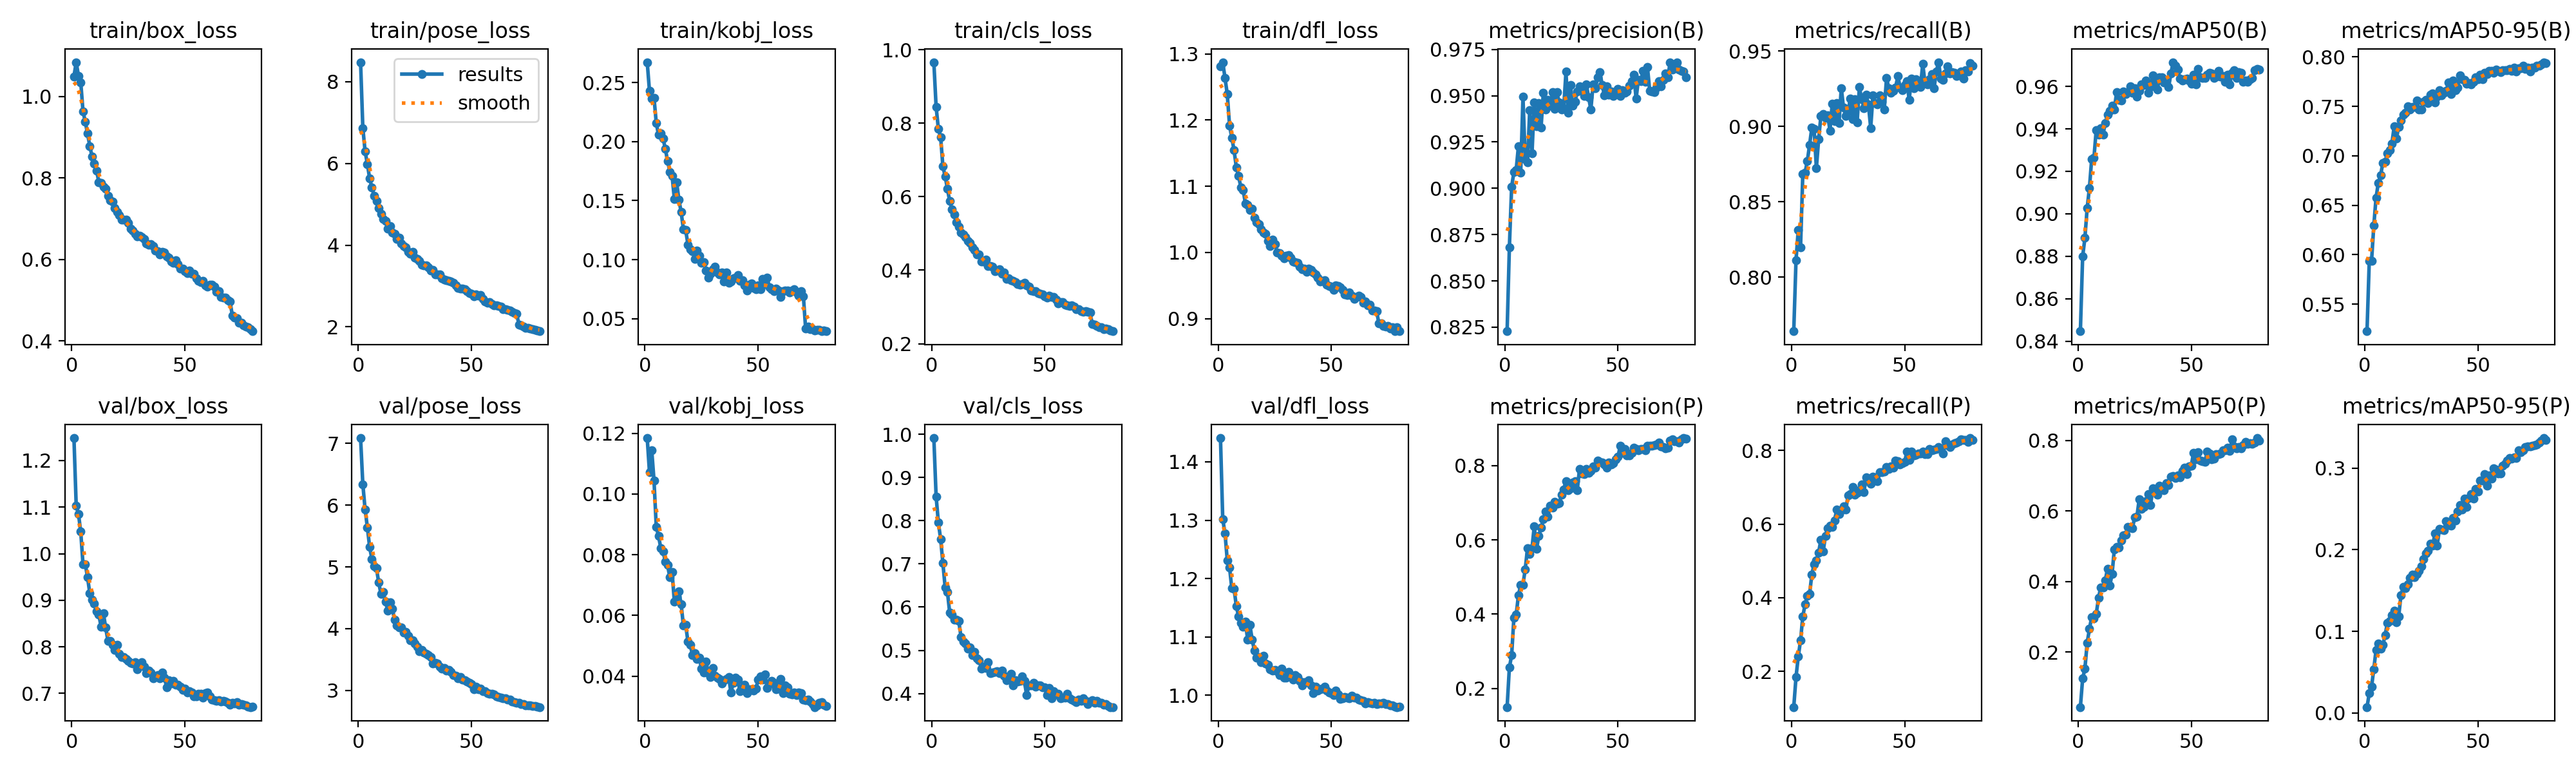
\includegraphics[width=\textwidth]{assets/images/results.png}
  \caption{Các đường loss và metric trong quá trình huấn luyện}
  \label{fig:train_results}
\end{figure}

Ở epoch đầu tiên, \texttt{train/box\_loss} là 1.04946 và giảm còn 0.42387 tại epoch 80.
Tương tự, \texttt{train/pose\_loss} giảm từ 8.47728 xuống 1.8933, còn \texttt{train/cls\_loss} giảm từ 0.96578 xuống 0.23405.
Trên tập validation, \texttt{val/box\_loss} giảm từ 1.24823 xuống 0.67094 và \texttt{val/pose\_loss} giảm từ 7.08597 xuống 2.7294.
Điều này cho thấy quá trình fine-tune toàn bộ mô hình vẫn giữ được xu hướng hội tụ ổn định.

\subsubsection{Phân tích metric trên tập validation}
Các chỉ số mAP trên tập validation tăng rõ rệt qua quá trình train.
Bảng~\ref{tab:val_progress} tóm tắt một số mốc epoch đại diện.

\begin{table}[H]
  \centering
  \caption{Một số mốc kết quả validation trong quá trình train}
  \label{tab:val_progress}
  \resizebox{\textwidth}{!}{%
  \begin{tabular}{@{}ccccc@{}}
    \toprule
    \textbf{Epoch} & \textbf{Box mAP@50} & \textbf{Box mAP@50-95} & \textbf{Pose mAP@50} & \textbf{Pose mAP@50-95} \\
    \midrule
    1  & 0.84473 & 0.52267 & 0.04447 & 0.00730 \\
    10 & 0.94044 & 0.70225 & 0.38398 & 0.11060 \\
    20 & 0.95758 & 0.74711 & 0.53198 & 0.16536 \\
    40 & 0.95969 & 0.76614 & 0.67366 & 0.23544 \\
    60 & 0.96387 & 0.78490 & 0.74778 & 0.29346 \\
    80 & 0.96784 & 0.79375 & 0.79959 & 0.33453 \\
    \bottomrule
  \end{tabular}%
  }
\end{table}

Nhánh Box đạt mAP@50 cao ngay từ các epoch đầu do mô hình pretrained đã có khả năng phát hiện người tương đối tốt.
Ngược lại, nhánh Pose tăng chậm hơn vì mô hình phải thích nghi với cấu trúc 18 keypoints của dataset, trong đó có thêm điểm \textit{Neck} so với chuẩn COCO 17 keypoints.
Tại epoch 80, validation đạt Box mAP@50 là 0.96784 và Pose mAP@50 là 0.79959.

\subsection{Kết quả đánh giá định lượng trên tập kiểm thử độc lập}
\label{subsec:quantitative_evaluation}
Sau khi huấn luyện, trọng số tốt nhất \texttt{best.pt} được đánh giá lại trên test split trong thư mục \texttt{sleeping-as-fall-lan3-test}.
Tập test gồm 616 ảnh và 984 instances, trong đó có 592 instances \texttt{no\_fall} và 392 instances \texttt{fall}.
Kết quả tổng hợp được trình bày trong Bảng~\ref{tab:results}.

\begin{table}[H]
  \centering
  \caption{Kết quả đánh giá định lượng mô hình trên tập dữ liệu kiểm thử độc lập}
  \label{tab:results}
  \resizebox{\textwidth}{!}{%
  \begin{tabular}{lcccccccc}
    \toprule
    \multirow{2}{*}{\textbf{Mô hình thực nghiệm}} & \multicolumn{4}{c}{\textbf{Tác vụ Nhận diện Vùng chứa (Box)}} & \multicolumn{4}{c}{\textbf{Tác vụ Ước lượng Tư thế (Pose)}} \\ \cline{2-9} 
     & \textbf{mAP@50} & \textbf{mAP@50-95} & \textbf{Precision} & \textbf{Recall} & \textbf{mAP@50} & \textbf{mAP@50-95} & \textbf{Precision} & \textbf{Recall} \\
    \midrule
    \textbf{\texttt{best.pt} trên test} & \textbf{95.7\%} & \textbf{76.9\%} & \textbf{97.4\%} & \textbf{93.9\%} & \textbf{69.4\%} & \textbf{29.1\%} & \textbf{79.7\%} & \textbf{75.9\%} \\
    \bottomrule
  \end{tabular}%
  }
\end{table}

Kết quả test cho thấy mô hình phát hiện hộp bao người khá tốt, với Box mAP@50 đạt 95.7\% và Recall đạt 93.9\%.
Đối với tác vụ keypoint, Pose mAP@50 đạt 69.4\%.
Mức này thấp hơn Box mAP@50 vì việc dự đoán chính xác 18 keypoints khó hơn so với chỉ định vị bounding box, đặc biệt trong các tư thế té ngã bị che khuất hoặc nằm sát nền.

\begin{table}[H]
  \centering
  \caption{Kết quả chi tiết theo class trên tập test}
  \label{tab:test_per_class}
  \resizebox{\textwidth}{!}{%
  \begin{tabular}{lcccccccc}
    \toprule
    \multirow{2}{*}{\textbf{Class}} & \multicolumn{4}{c}{\textbf{Box}} & \multicolumn{4}{c}{\textbf{Pose}} \\ \cline{2-9}
    & \textbf{P} & \textbf{R} & \textbf{mAP@50} & \textbf{mAP@50-95} & \textbf{P} & \textbf{R} & \textbf{mAP@50} & \textbf{mAP@50-95} \\
    \midrule
    \texttt{no\_fall} & 96.7\% & 92.9\% & 94.4\% & 74.0\% & 89.1\% & 84.5\% & 81.1\% & 41.1\% \\
    \texttt{fall}    & 98.0\% & 94.9\% & 96.9\% & 79.8\% & 70.4\% & 67.3\% & 57.6\% & 17.2\% \\
    \bottomrule
  \end{tabular}%
  }
\end{table}

Class \texttt{fall} có Box mAP@50 cao hơn \texttt{no\_fall}, cho thấy mô hình định vị người té ngã khá tốt.
Tuy nhiên, Pose mAP@50 của class \texttt{fall} chỉ đạt 57.6\%, thấp hơn \texttt{no\_fall}.
Điều này phù hợp với đặc thù bài toán: người té ngã thường có dáng nằm, co gập hoặc bị che khuất, làm cho keypoint khó khớp chính xác hơn.

\subsubsection{Phân tích đường cong precision-recall}
Đường cong Precision-Recall trực quan hóa quan hệ giữa precision và recall tại các ngưỡng confidence khác nhau.
Hình~\ref{fig:pr_curve} trình bày PR curve cho Box và Pose trên tập test.

\begin{figure}[H]
  \centering
  \begin{subfigure}[b]{0.48\textwidth}
    \centering
    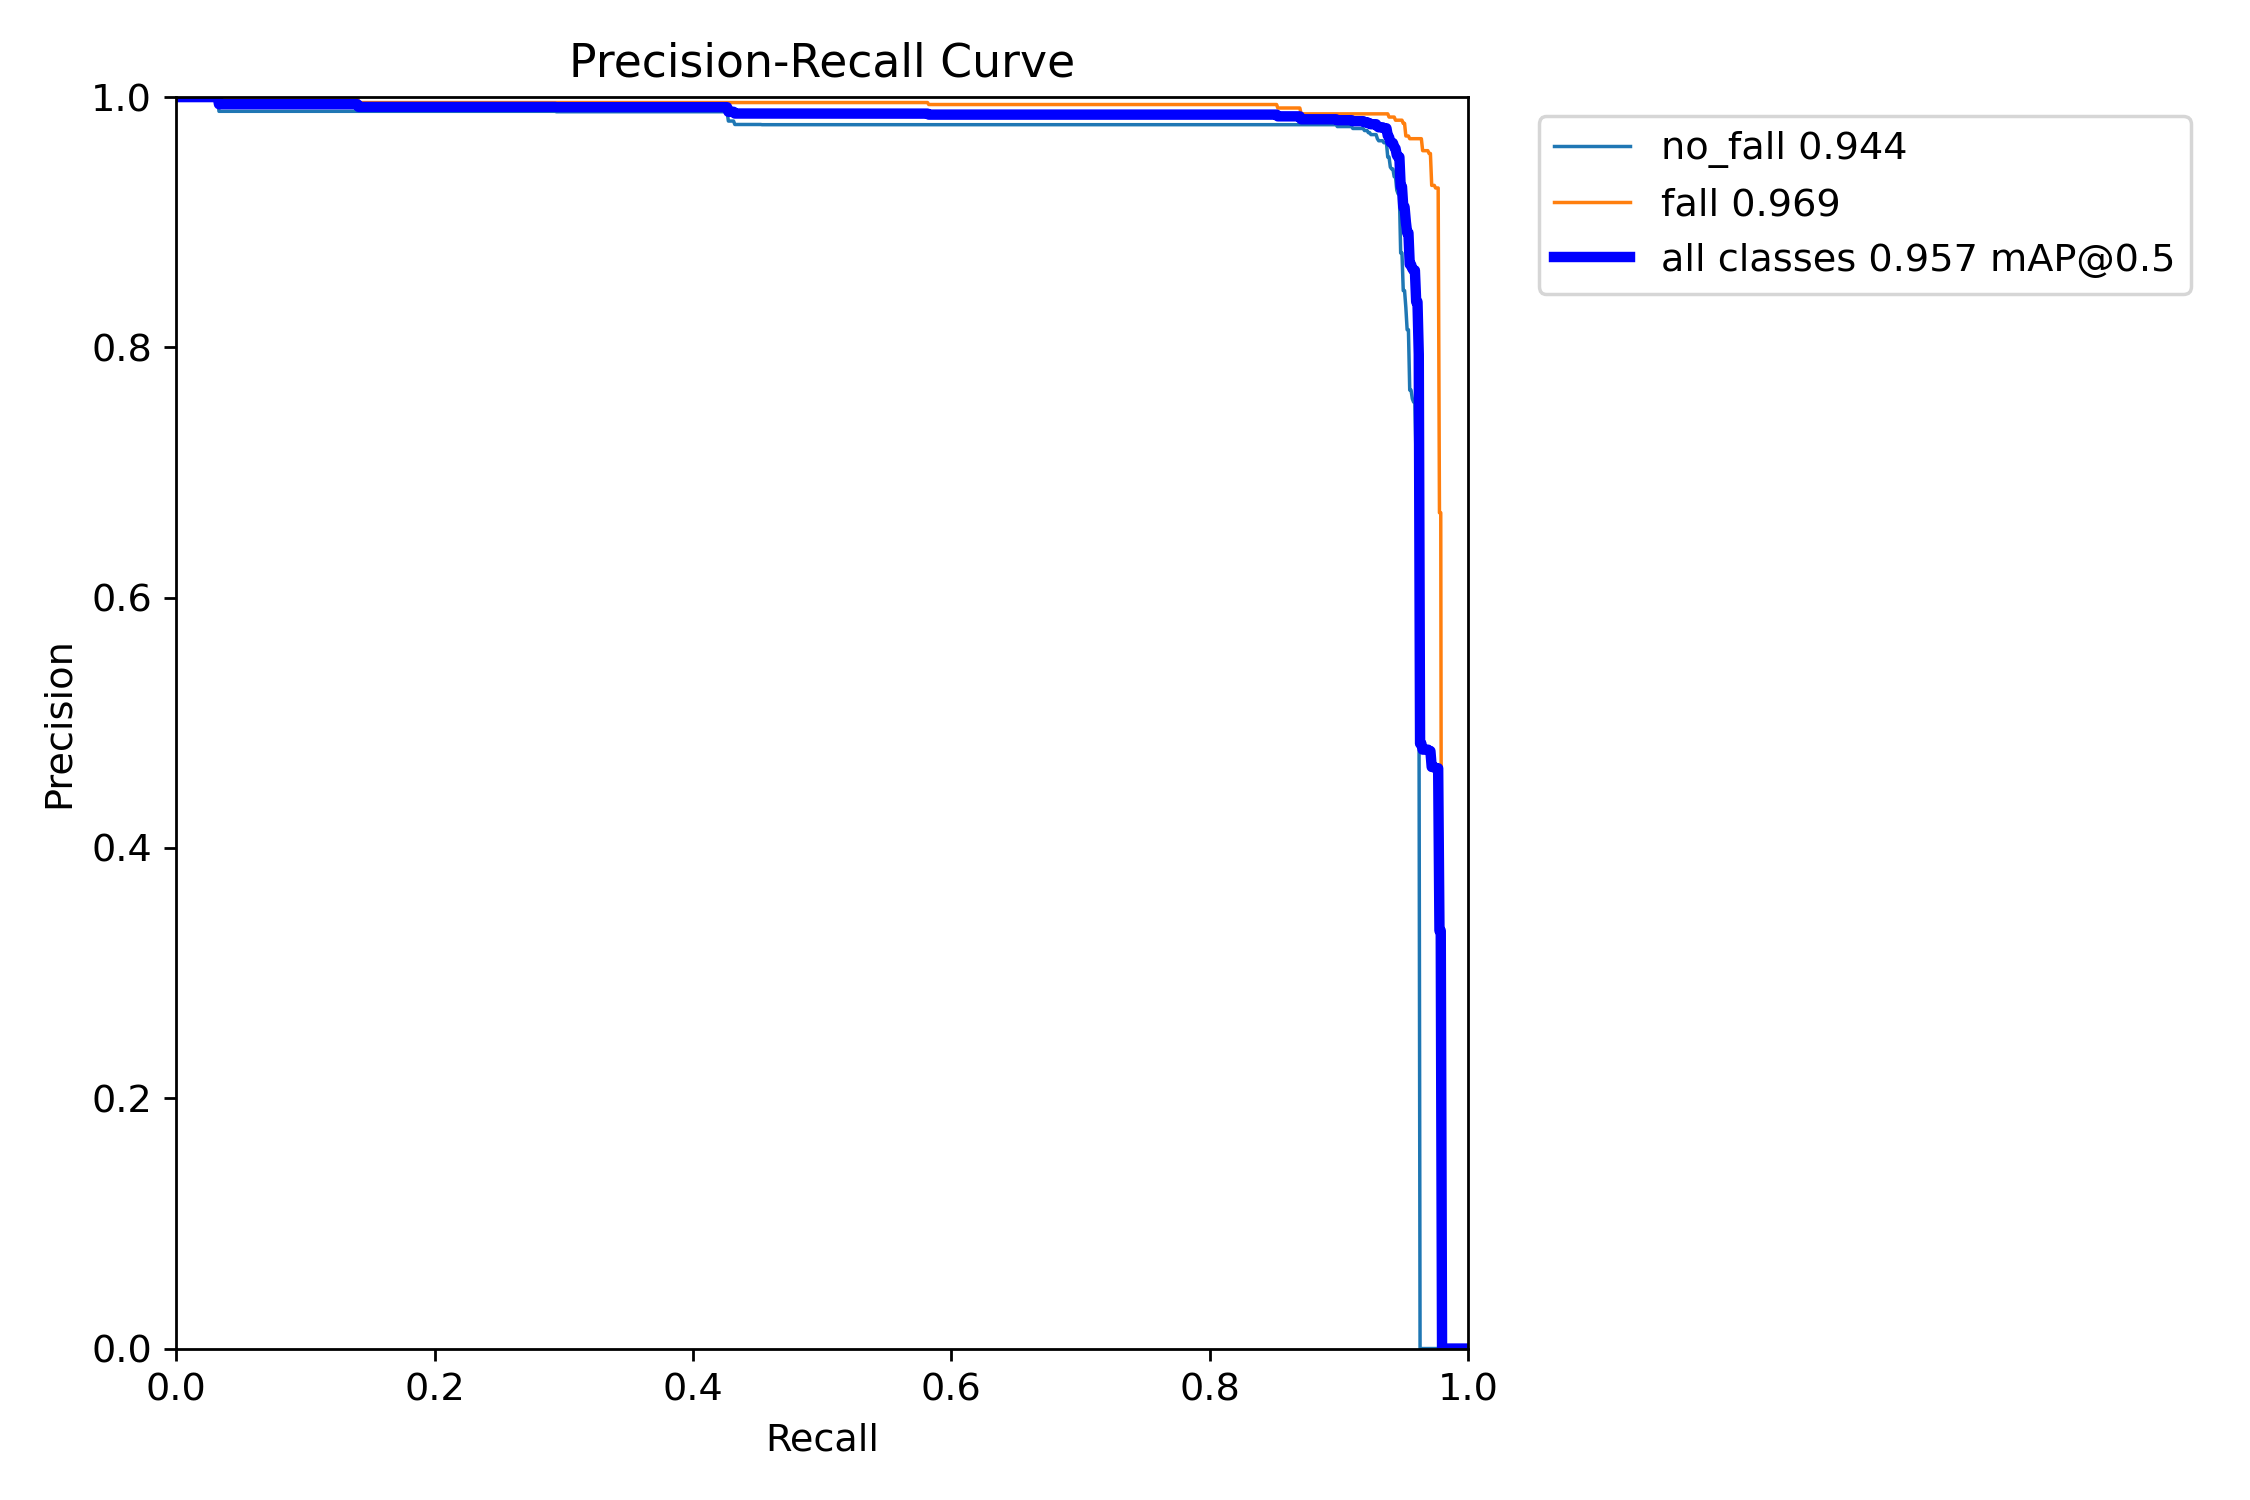
\includegraphics[width=\textwidth]{assets/images/BoxPR_curve.png}
    \caption{Box PR curve}
  \end{subfigure}
  \hfill
  \begin{subfigure}[b]{0.48\textwidth}
    \centering
    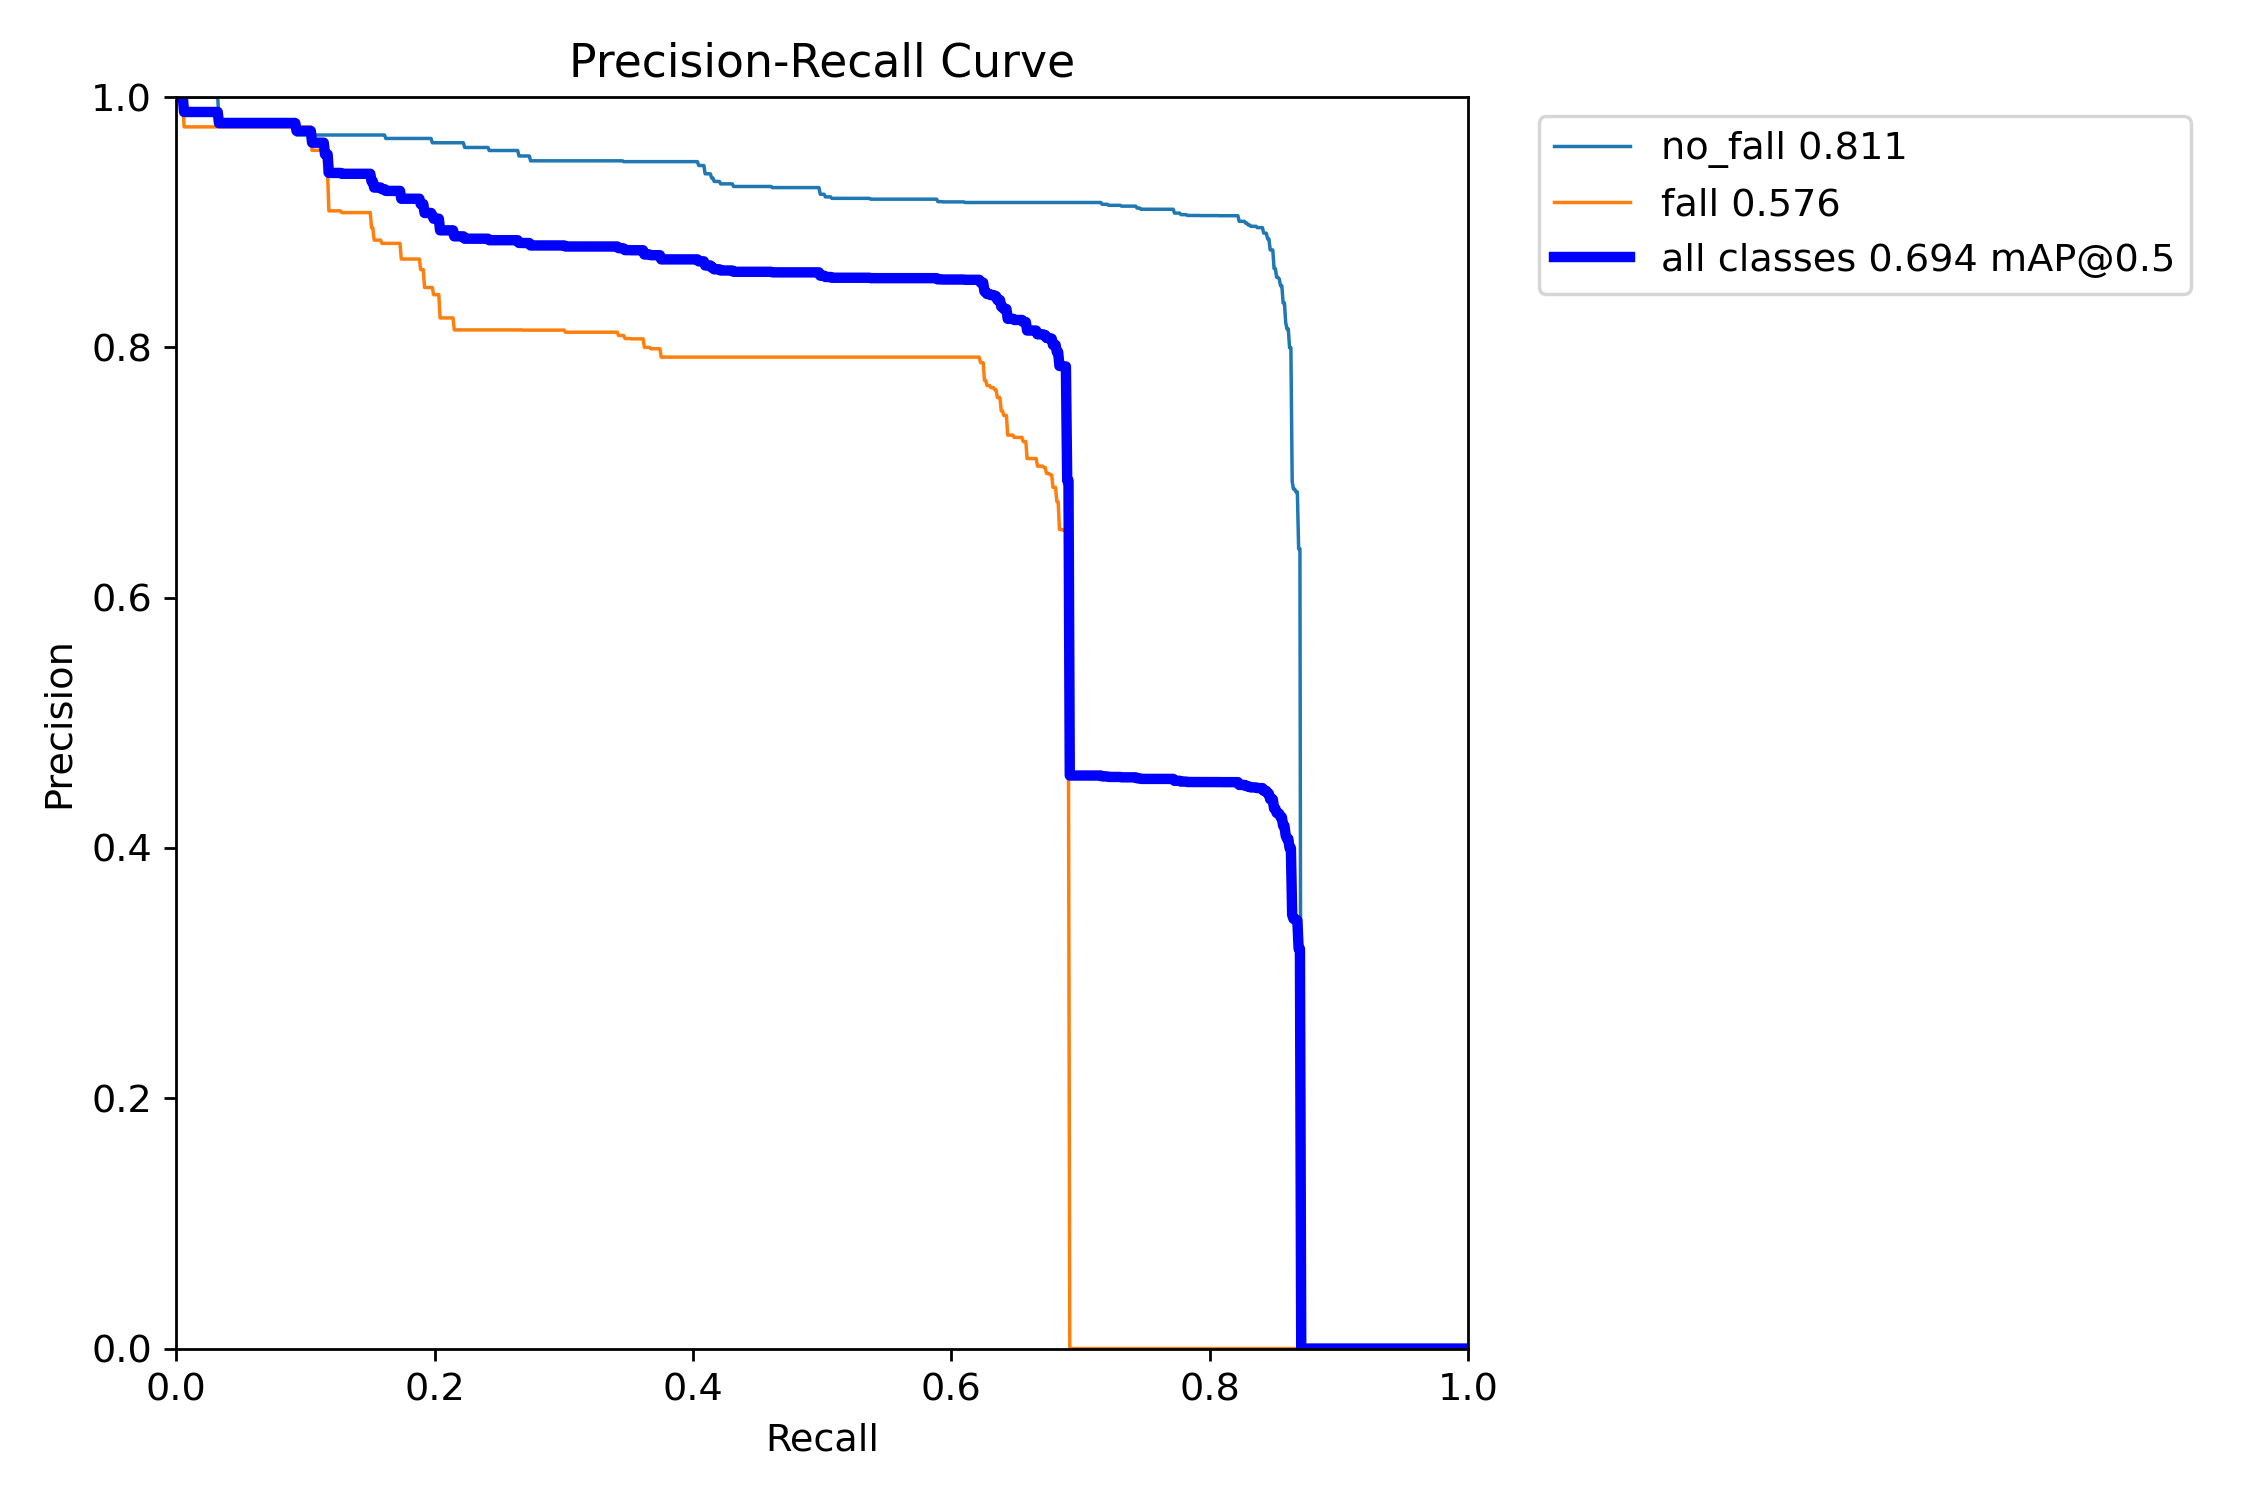
\includegraphics[width=\textwidth]{assets/images/PosePR_curve.png}
    \caption{Pose PR curve}
  \end{subfigure}
  \caption{Đường cong Precision-Recall trên tập test}
  \label{fig:pr_curve}
\end{figure}

Box PR curve có diện tích cao ở cả hai class, tương ứng với mAP@50 tổng hợp 0.957 trên tập test.
Pose PR curve thấp hơn, đặc biệt ở class \texttt{fall}, phản ánh khó khăn của bài toán keypoint khi cơ thể người nằm ngang hoặc bị che khuất.

\begin{figure}[H]
  \centering
  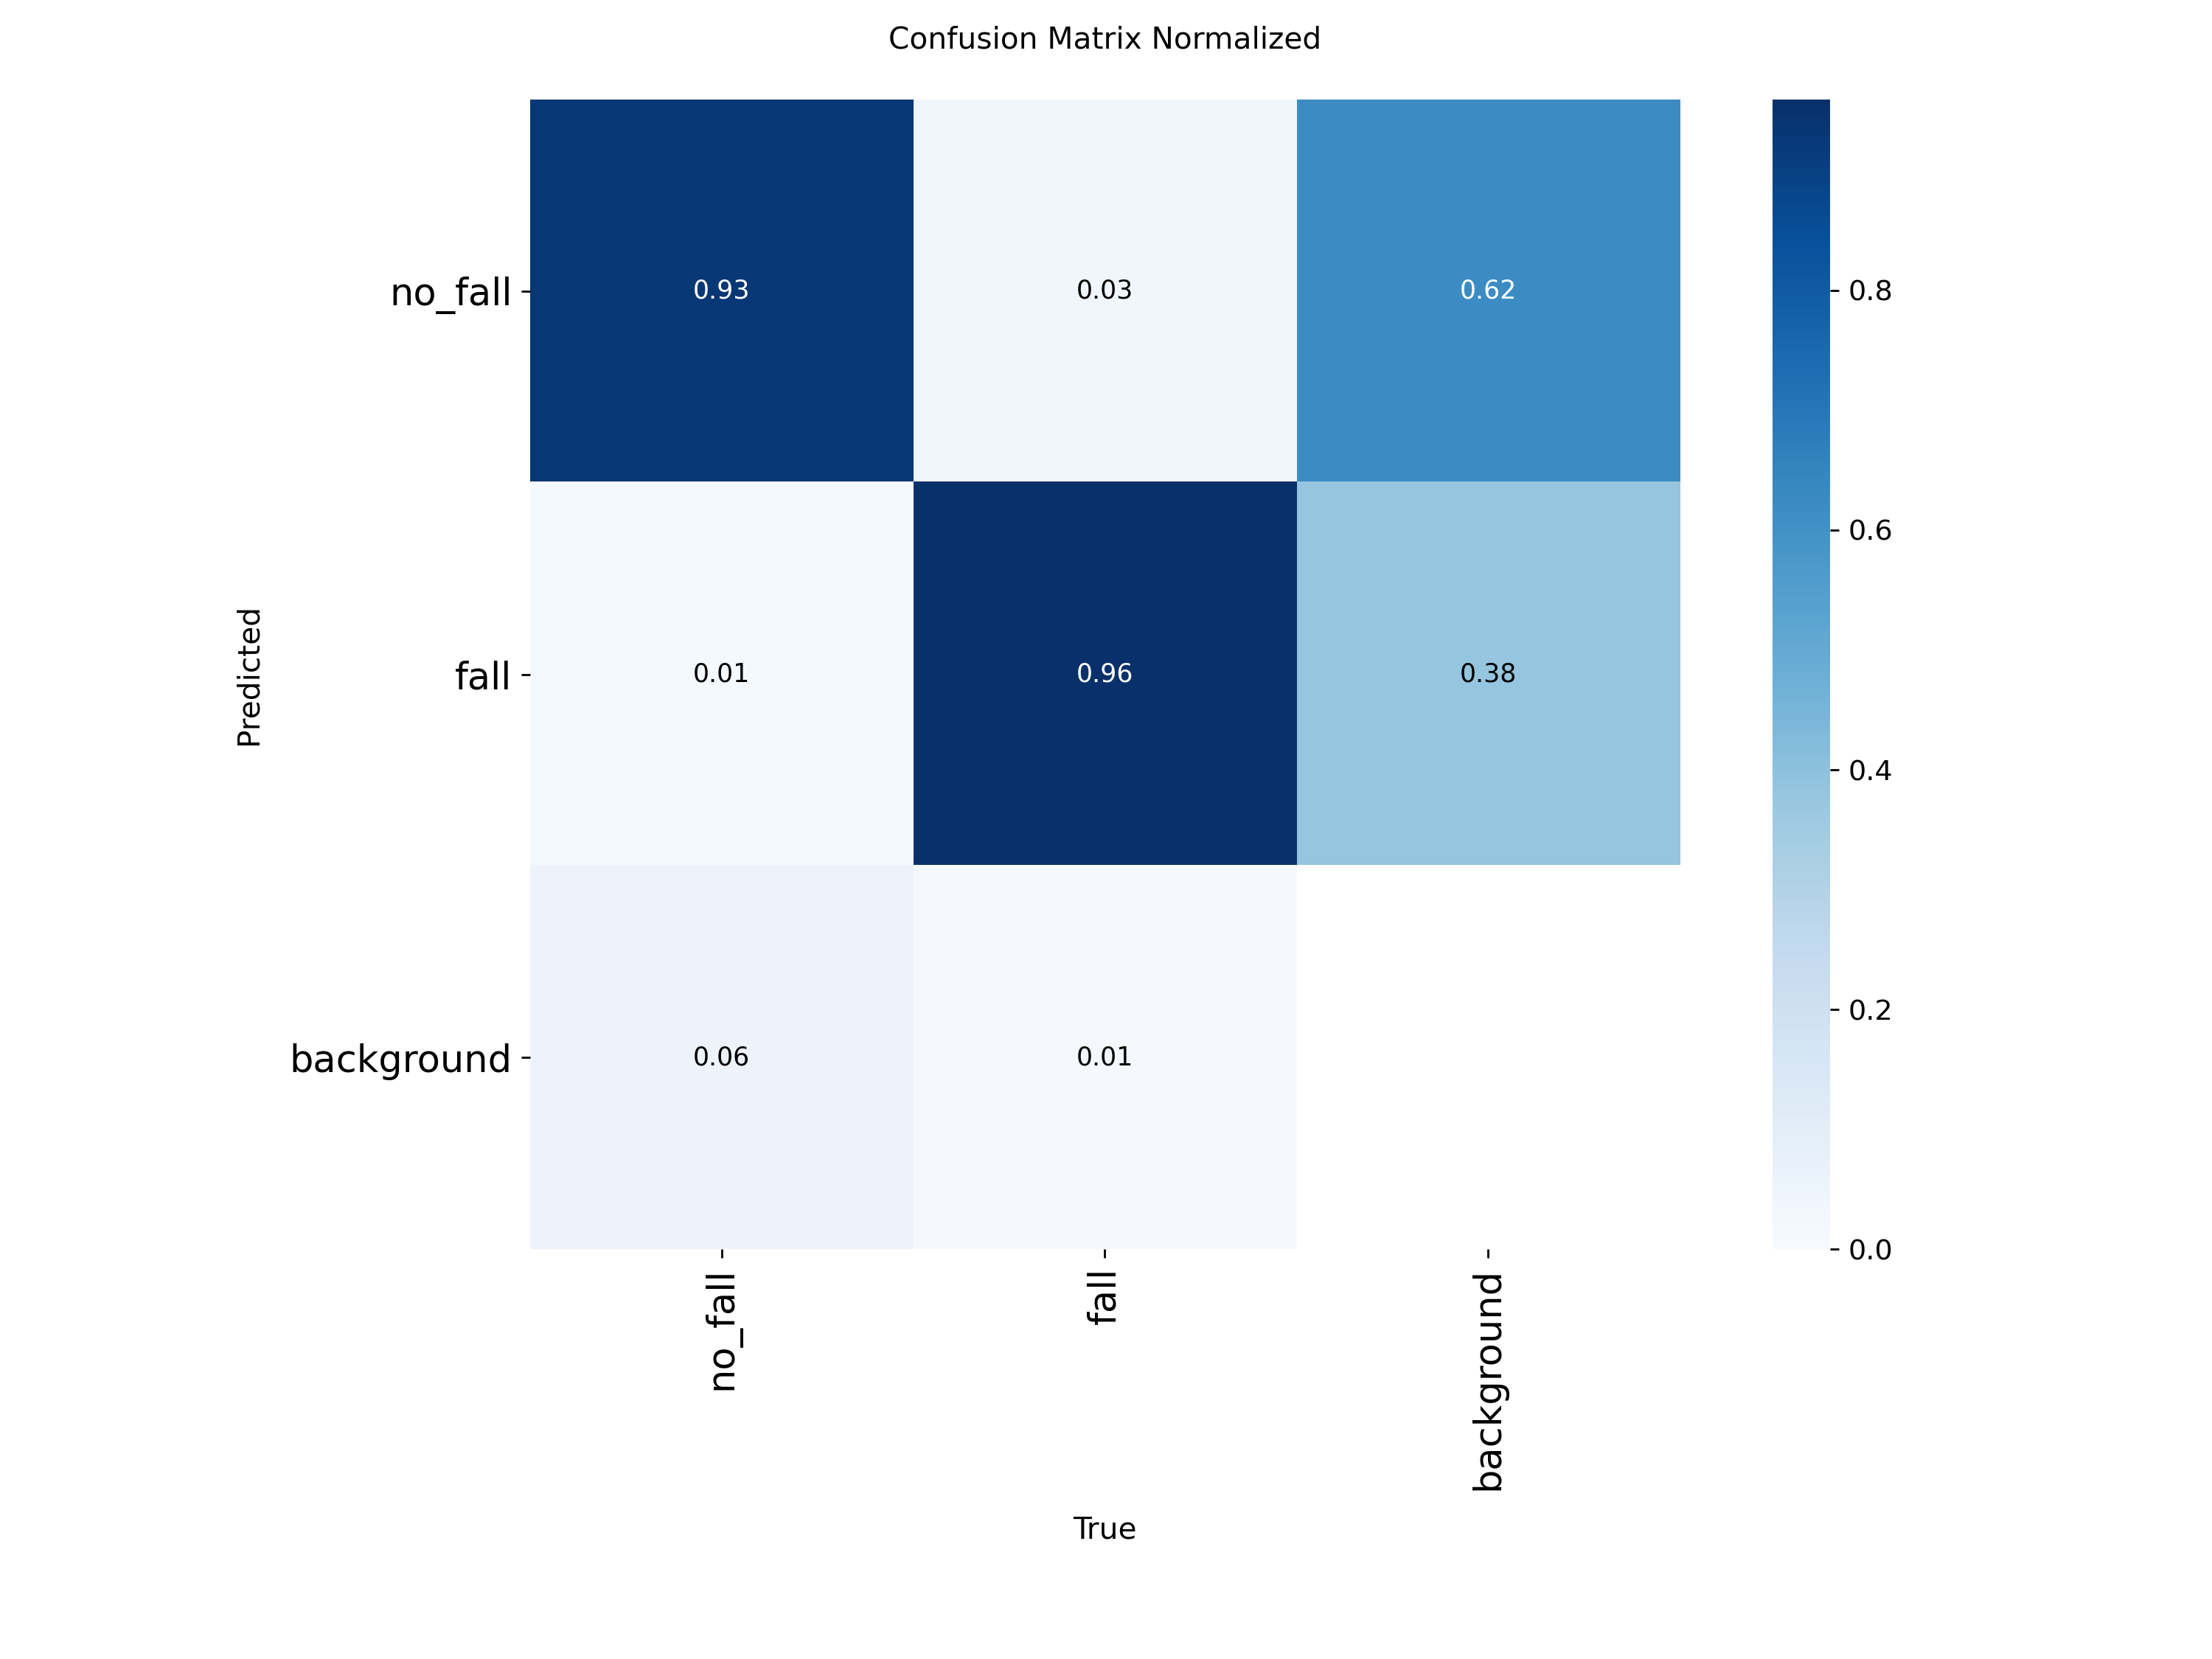
\includegraphics[width=0.72\textwidth]{assets/images/confusion_matrix_normalized.png}
  \caption{Confusion matrix chuẩn hóa trên tập test}
  \label{fig:test_confusion_matrix}
\end{figure}

\subsection{Phân tích định tính và kết quả thử nghiệm inference trực quan}
\label{subsec:qualitative_evaluation}
Ngoài các chỉ số định lượng, kết quả inference trực quan giúp kiểm tra cách mô hình dự đoán bounding box, class và keypoint trên từng ảnh.
Hình~\ref{fig:test_predictions} minh họa một số batch dự đoán trên test split sau khi validate bằng \texttt{best.pt}.

\begin{figure}[H]
  \centering
  \begin{subfigure}[b]{0.49\textwidth}
    \centering
    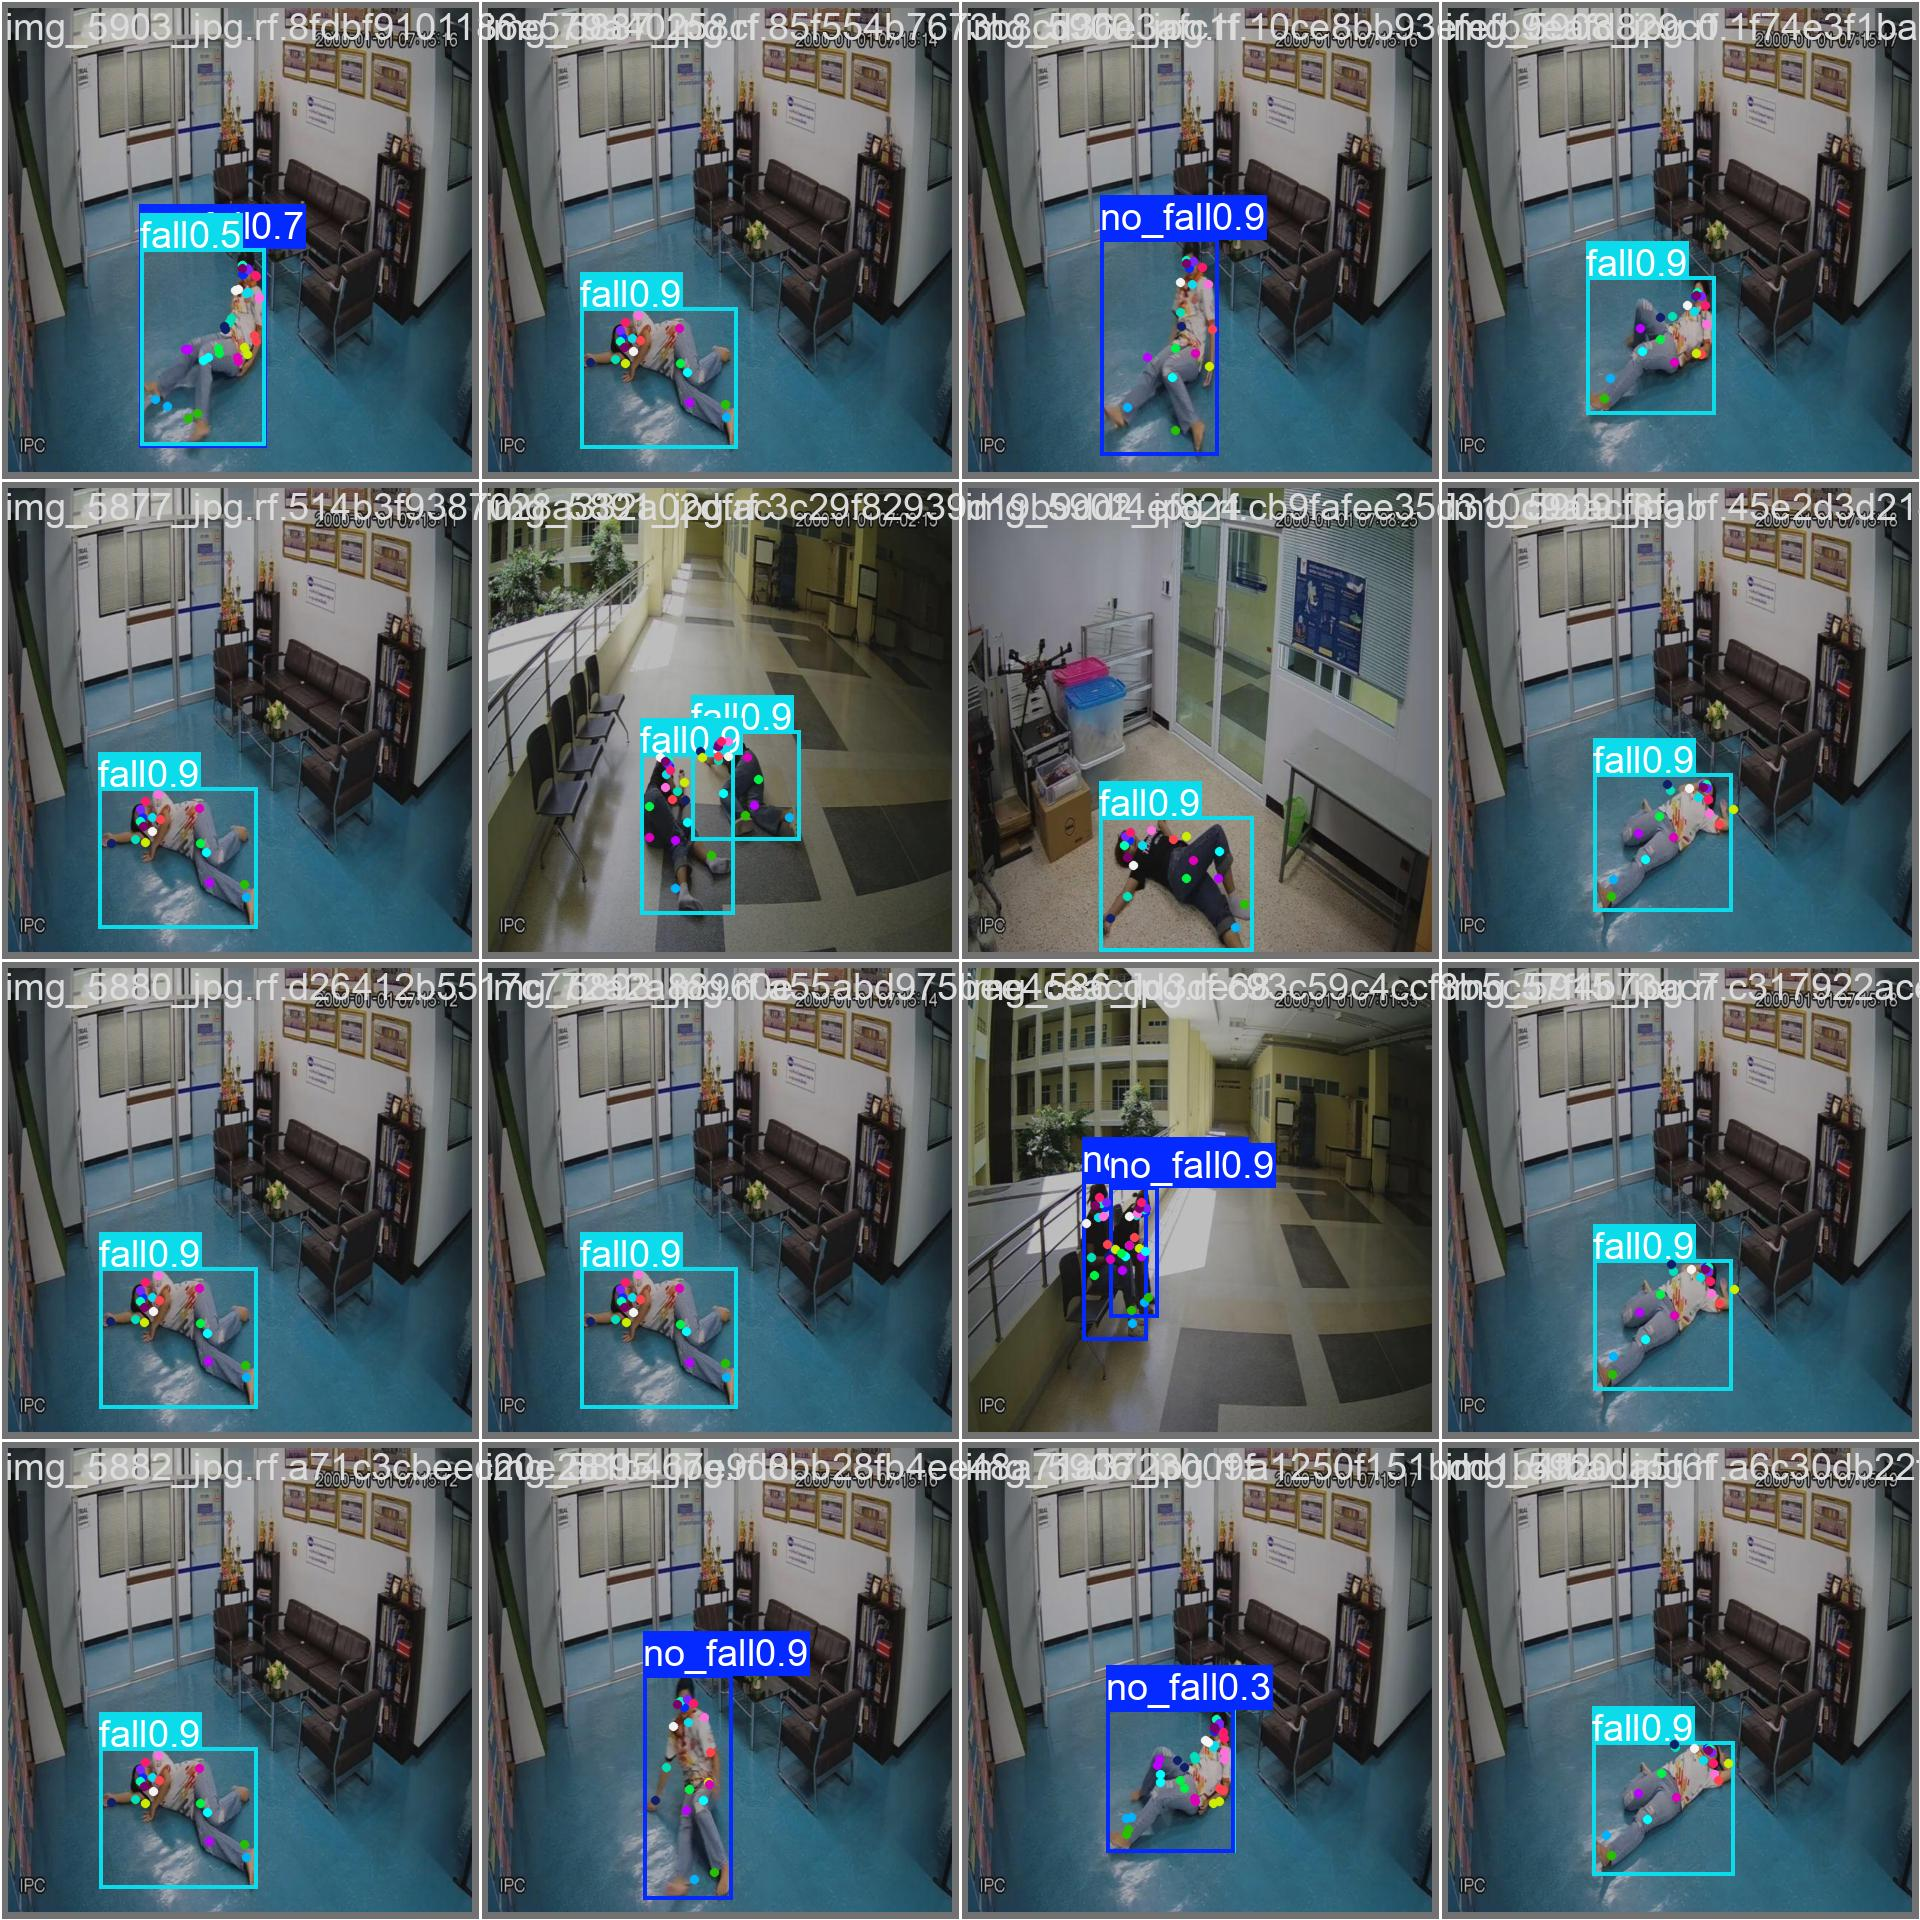
\includegraphics[width=\textwidth]{assets/images/val_batch0_pred.jpg}
    \caption{Batch dự đoán 1}
  \end{subfigure}
  \hfill
  \begin{subfigure}[b]{0.49\textwidth}
    \centering
    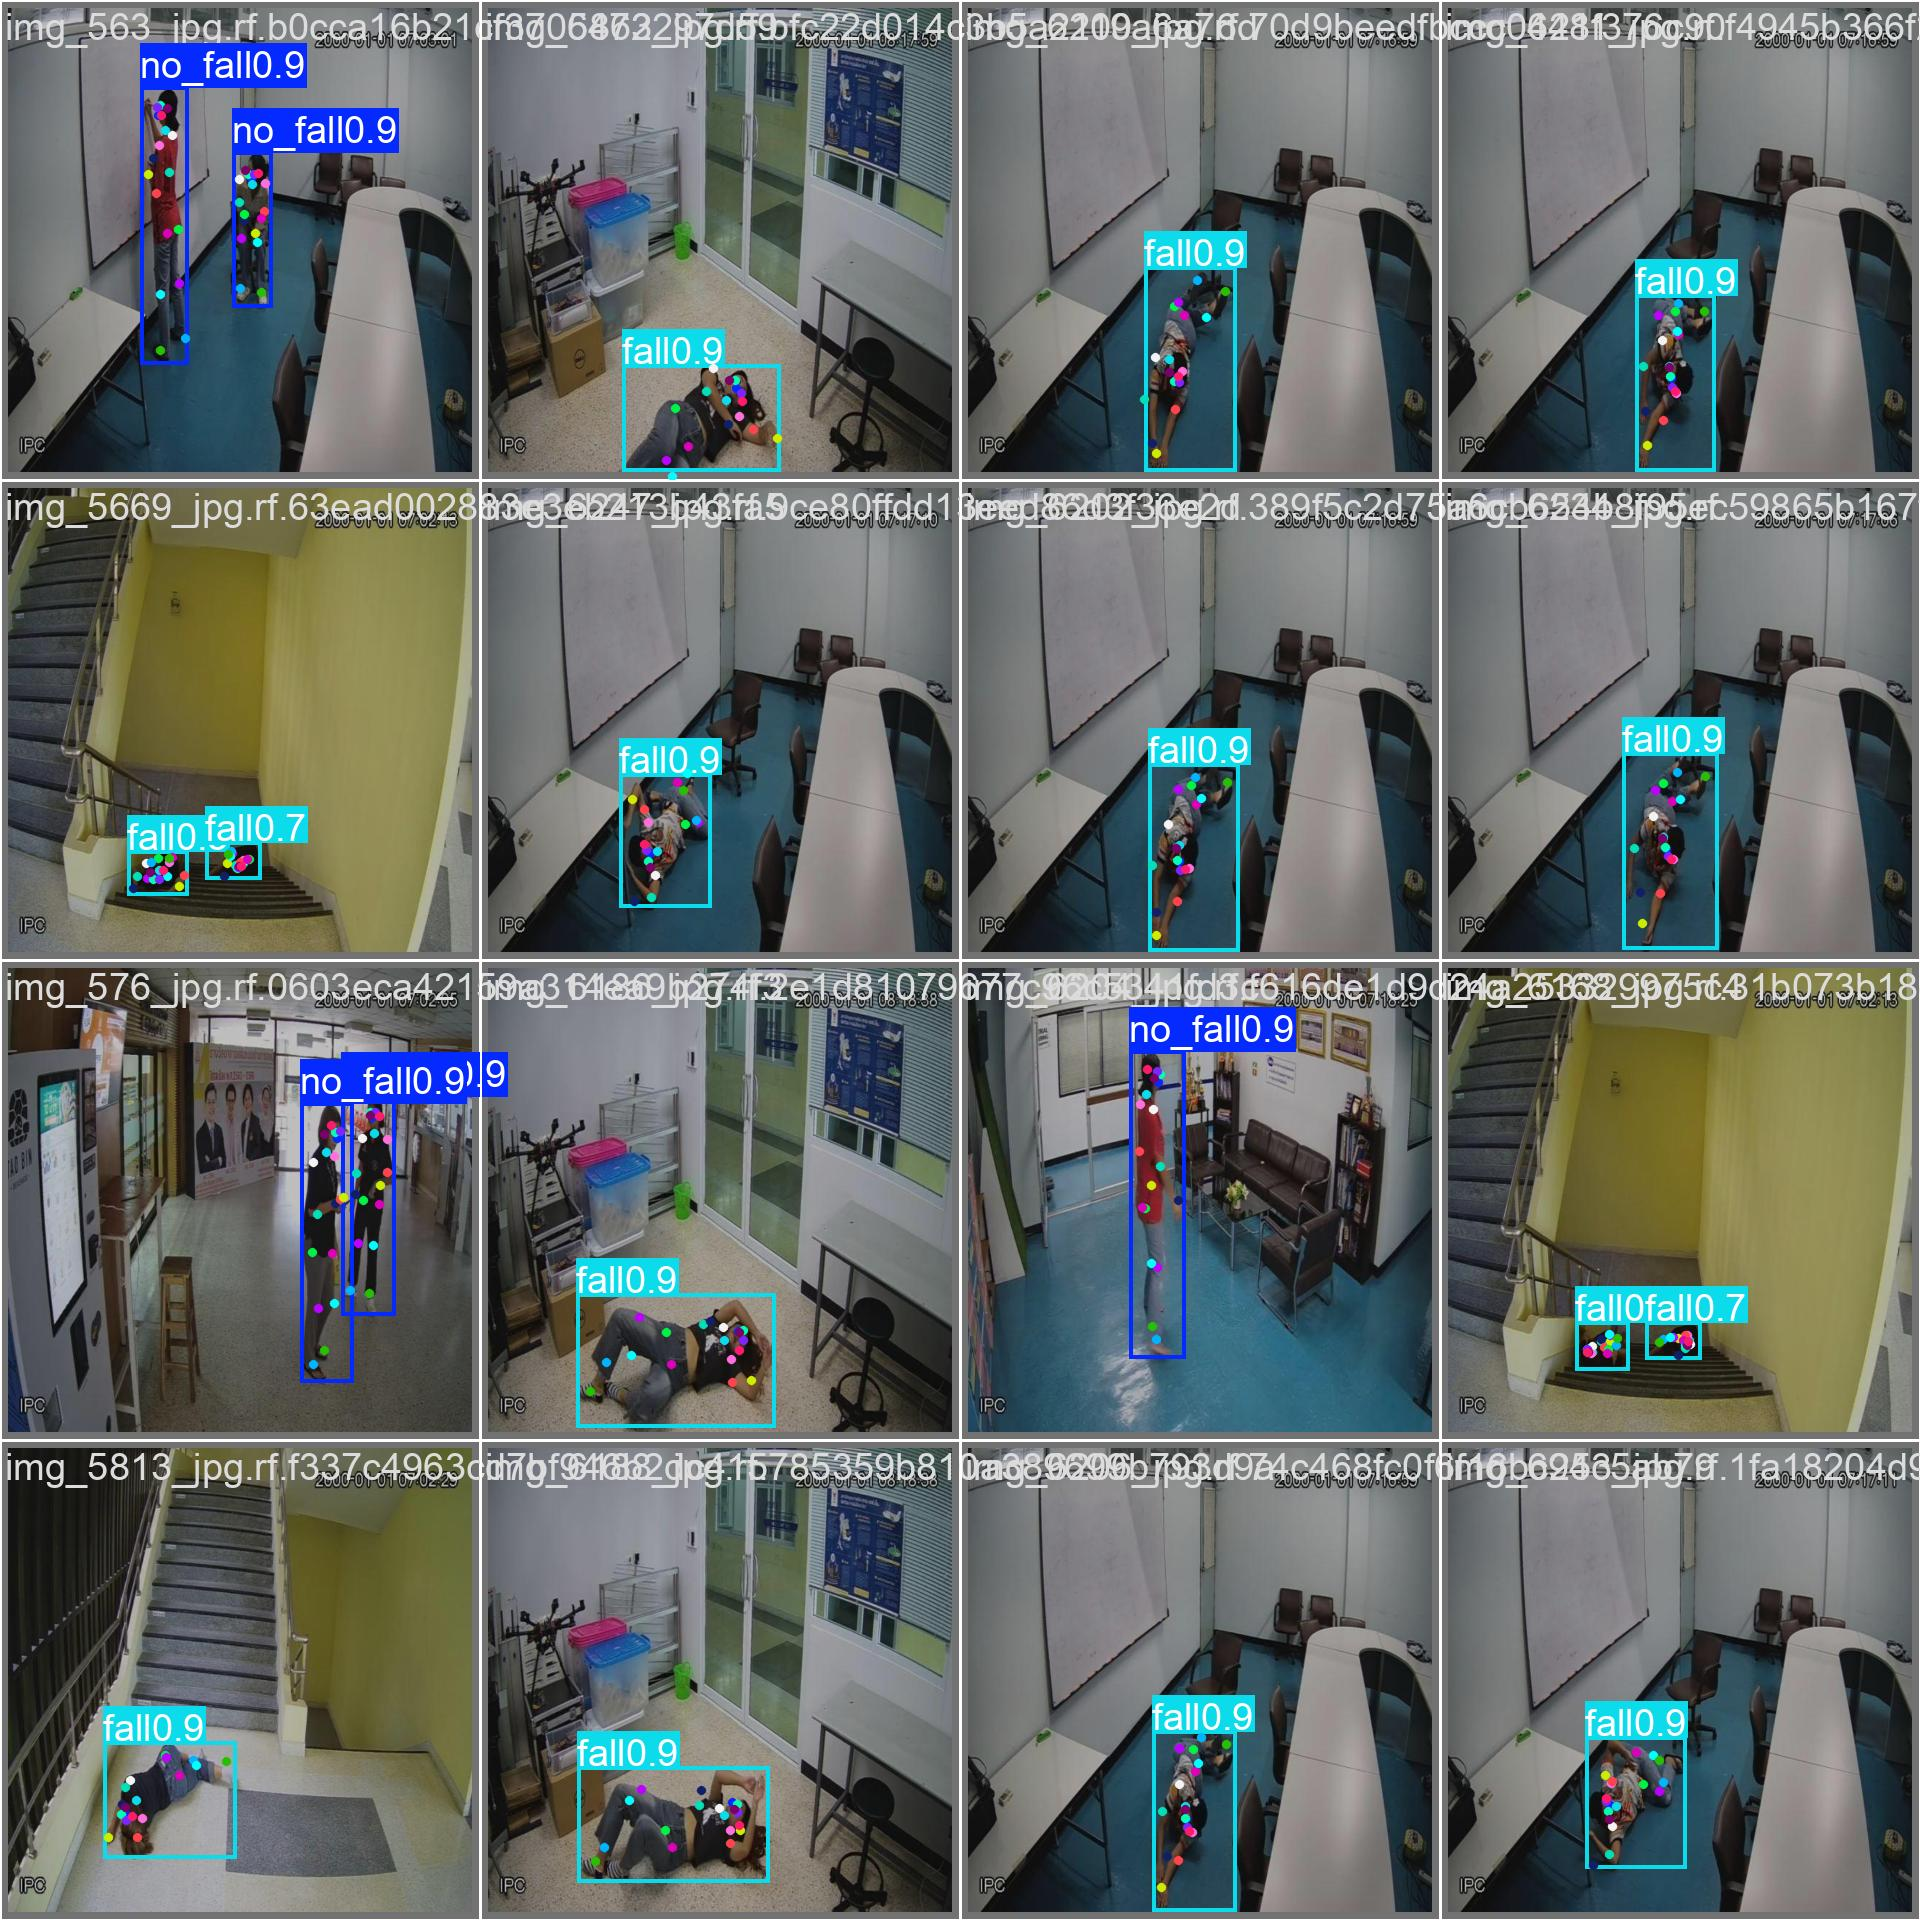
\includegraphics[width=\textwidth]{assets/images/val_batch2_pred.jpg}
    \caption{Batch dự đoán 2}
  \end{subfigure}
  \caption{Kết quả inference trực quan trên test split}
  \label{fig:test_predictions}
\end{figure}

Quan sát trực quan cho thấy mô hình nhận diện tốt nhiều trường hợp người nằm hoặc ngã trên sàn, với bounding box bao quanh đúng vùng cơ thể và nhãn \texttt{fall} có độ tin cậy cao.
Trong các ảnh có người đứng hoặc đi lại, mô hình thường dự đoán nhãn \texttt{no\_fall}, đồng thời keypoint vẫn bám theo cấu trúc cơ thể.
Điều này phù hợp với kết quả định lượng ở Bảng~\ref{tab:results}, trong đó Box mAP@50 trên tập test đạt 95.7\%.

Tuy nhiên, phần keypoint của class \texttt{fall} vẫn khó hơn so với class \texttt{no\_fall}.
Ở một số ảnh, người nằm ngang bị co gập, một phần cơ thể bị khuất bởi góc camera hoặc vật thể xung quanh, làm các điểm khớp bị chồng lên nhau hoặc không rõ ràng.
Đây là nguyên nhân khiến Pose mAP@50 của class \texttt{fall} chỉ đạt 57.6\%, thấp hơn đáng kể so với 81.1\% của class \texttt{no\_fall}.

\subsection{Phân tích chi tiết lỗi}
\label{subsec:error_analysis}
Từ kết quả test và các ảnh inference, có thể thấy lỗi của mô hình tập trung nhiều hơn ở phần pose/keypoint thay vì phần bounding box.
Box mAP@50 đạt 95.7\%, trong khi Pose mAP@50 đạt 69.4\%.
Sự chênh lệch này cho thấy mô hình định vị người khá tốt, nhưng việc đặt đúng toàn bộ 18 keypoints vẫn là phần khó hơn của bài toán.

\begin{itemize}
    \item \textbf{Nhầm lẫn giữa tư thế nằm và té ngã:} Dataset chủ động ánh xạ một phần class \textit{Sleeping} vào \texttt{fall}. Cách làm này giúp tăng số mẫu cho nhóm \texttt{fall}, nhưng cũng làm biên phân biệt giữa té ngã thật và trạng thái nằm/ngủ trở nên khó hơn. Vì vậy, khi triển khai thực tế cần kết hợp thêm hậu xử lý theo thời gian để giảm cảnh báo sai.
    \item \textbf{Che khuất và góc nhìn camera:} Nhiều ảnh được chụp từ camera giám sát góc cao hoặc góc chéo. Khi người nằm sát sàn, co gập hoặc bị vật thể che khuất, các khớp như cổ tay, cổ chân, đầu gối dễ bị mờ hoặc chồng lên nhau. Trường hợp này ảnh hưởng trực tiếp đến OKS và làm Pose mAP của class \texttt{fall} thấp hơn.
    \item \textbf{Nhiều người trong cùng ảnh:} Một số ảnh có nhiều người đứng gần nhau hoặc nhiều người ngã trong cùng khung hình. Khi bounding box giao nhau, keypoint của các đối tượng có thể bị gán gần nhau, dẫn đến dự đoán trùng lặp hoặc sai một phần cấu trúc khung xương.
    \item \textbf{Độ khó khác nhau giữa Box và Pose:} Kết quả ở Bảng~\ref{tab:test_per_class} cho thấy class \texttt{fall} đạt Box mAP@50 96.9\%, nhưng Pose mAP@50 chỉ đạt 57.6\%. Điều này cho thấy mô hình vẫn phát hiện được người té ngã, nhưng độ chính xác keypoint bị ảnh hưởng bởi tư thế nằm ngang và mức độ che khuất.
\end{itemize}

Từ các lỗi trên, hướng cải thiện phù hợp là bổ sung dữ liệu té ngã ở nhiều góc nhìn hơn, đặc biệt là các tình huống bị che khuất một phần.
Ngoài ra, khi triển khai phần mềm nhận diện, nên kết hợp kết quả từng frame với thông tin theo thời gian như trạng thái trước đó, độ ổn định của nhãn \texttt{fall}, tỷ lệ chiều rộng/chiều cao của bounding box và vị trí tương đối của các keypoint chính.

\section{Kết luận và hướng phát triển}
\label{sec:conclusion}

\subsection{Kết luận}
Đề tài đã thực hiện quá trình fine-tune mô hình \texttt{yolo11s-pose.pt} cho bài toán phát hiện té ngã dựa trên tư thế người.
Quy trình thực hiện bao gồm chuẩn bị dataset theo định dạng YOLO Pose, chuyển bài toán về hai lớp \texttt{fall} và \texttt{no\_fall}, cấu hình huấn luyện trên Kaggle, fine-tune toàn bộ mô hình và đánh giá lại trên tập kiểm thử độc lập.
Các nội dung chính đã đạt được gồm:
\begin{itemize}[nosep]
  \item Trình bày cơ sở lý thuyết về Object Detection, YOLO11-Pose, Human Pose Estimation, các hàm loss và các độ đo đánh giá liên quan.
  \item Xây dựng và kiểm tra dataset dạng keypoint với 18 điểm tư thế, trong đó lớp \texttt{sleeping} được ánh xạ có chủ đích sang lớp \texttt{fall}.
  \item Thiết lập pipeline fine-tune với mô hình \texttt{yolo11s-pose.pt}, kích thước ảnh \texttt{960}, batch size \texttt{8}, optimizer AdamW và huấn luyện tối đa \texttt{80} epoch.
  \item Đánh giá mô hình trên tập test gồm \texttt{616} ảnh và \texttt{984} đối tượng, đạt Box mAP@50 là \texttt{95.7\%}, Box mAP@50--95 là \texttt{76.9\%}, Pose mAP@50 là \texttt{69.4\%} và Pose mAP@50--95 là \texttt{29.1\%}.
\end{itemize}

Kết quả cho thấy mô hình có khả năng phát hiện vùng người tương đối tốt trong cả hai lớp \texttt{fall} và \texttt{no\_fall}.
Đối với bài toán phát hiện té ngã, kết quả Box của lớp \texttt{fall} đạt mAP@50 khoảng \texttt{96.9\%}, cho thấy mô hình nhận diện được phần lớn các trường hợp người nằm hoặc ngã trong ảnh.
Tuy nhiên, phần ước lượng keypoint vẫn khó hơn rõ rệt, đặc biệt ở lớp \texttt{fall}, do cơ thể thường bị co lại, nằm ngang, che khuất một phần hoặc xuất hiện trong các góc chụp không thuận lợi.
Vì vậy, mô hình phù hợp để làm thành phần nhận diện ban đầu trong hệ thống phát hiện té ngã, nhưng khi triển khai thực tế cần kết hợp thêm hậu xử lý theo thời gian để giảm nhầm lẫn giữa ngủ, nằm nghỉ và té ngã.

\subsection{Hạn chế}
\begin{itemize}[nosep]
  \item Dataset tuy đã được xử lý lại nhưng vẫn còn phụ thuộc vào dữ liệu ảnh tĩnh, chưa phản ánh đầy đủ chuyển động trước và sau khi té ngã.
  \item Việc ánh xạ lớp \texttt{sleeping} sang \texttt{fall} giúp tăng số lượng mẫu cho lớp té ngã, nhưng cũng làm mô hình dễ nhầm các tư thế nằm nghỉ với tình huống té ngã thật nếu chỉ xét từng frame đơn lẻ.
  \item Kết quả Pose của lớp \texttt{fall} còn thấp hơn lớp \texttt{no\_fall}, đặc biệt ở mAP@50--95, cho thấy việc định vị chính xác keypoint trong các tư thế ngã vẫn là điểm khó.
  \item Mô hình mới được đánh giá chủ yếu trên tập ảnh kiểm thử, chưa có đánh giá đầy đủ trên video thực tế theo thời gian dài.
  \item Đề tài chưa đi sâu vào tối ưu tốc độ suy luận, kích thước mô hình và khả năng triển khai trên thiết bị edge hoặc camera có tài nguyên hạn chế.
\end{itemize}

\subsection{Hướng phát triển}
\begin{itemize}[nosep]
  \item Bổ sung dữ liệu ở nhiều bối cảnh hơn như phòng ngủ, bệnh viện, hành lang, cầu thang và các góc camera từ trên cao, ngang người hoặc góc chéo.
  \item Tách rõ hơn các tình huống \texttt{fall}, \texttt{sleeping} và \texttt{lying} nếu có đủ dữ liệu, hoặc giữ mô hình hai lớp nhưng bổ sung tầng hậu xử lý để kiểm tra trạng thái theo thời gian.
  \item Kết hợp thông tin temporal từ video, chẳng hạn theo dõi sự thay đổi tư thế qua nhiều frame, thời gian duy trì nhãn \texttt{fall}, tốc độ thay đổi bounding box và vị trí tương đối của các keypoint chính.
  \item Thử nghiệm thêm các kích thước mô hình khác như \texttt{yolo11m-pose.pt} hoặc \texttt{yolo11l-pose.pt} để so sánh giữa độ chính xác và tốc độ suy luận.
  \item Tối ưu mô hình bằng các kỹ thuật như quantization, pruning hoặc export sang ONNX/TensorRT để phục vụ triển khai thực tế.
  \item Xây dựng và đánh giá hệ thống nhận diện hoàn chỉnh trên video, trong đó kết quả từ YOLO11-Pose được kết hợp với luật hậu xử lý nhằm giảm cảnh báo sai.
\end{itemize}

% ============================================================
%  TÀI LIỆU THAM KHẢO
% ============================================================
\newpage
\begin{thebibliography}{99}

\bibitem{redmon2016yolo}
J. Redmon, S. Divvala, R. Girshick, and A. Farhadi,
``You Only Look Once: Unified, Real-Time Object Detection,''
in \textit{Proc. IEEE CVPR}, 2016, pp. 779--788.

\bibitem{ren2015faster}
S. Ren, K. He, R. Girshick, and J. Sun,
``Faster R-CNN: Towards Real-Time Object Detection with Region Proposal Networks,''
in \textit{Advances in Neural Information Processing Systems (NeurIPS)}, 2015.

\bibitem{li2020generalized}
X. Li \textit{et al.},
``Generalized Focal Loss: Learning Qualified and Distributed Bounding Boxes for Dense Object Detection,''
in \textit{Advances in Neural Information Processing Systems (NeurIPS)}, 2020.

\bibitem{lin2014coco}
T.-Y. Lin \textit{et al.},
``Microsoft COCO: Common Objects in Context,''
in \textit{Proc. ECCV}, 2014.

\bibitem{ultralytics2024yolo11}
Ultralytics,
``YOLO11: State-of-the-Art Object Detection,''
\url{https://github.com/ultralytics/ultralytics}, 2024.

\bibitem{cao2017openpose}
Z. Cao, T. Simon, S.-E. Wei, and Y. Sheikh,
``Realtime Multi-Person 2D Pose Estimation using Part Affinity Fields,''
in \textit{Proc. IEEE CVPR}, 2017.

\end{thebibliography}

\end{document}
